% This template has been tested with LLNCS DOCUMENT CLASS -- version 2.20 (10-Mar-2018)

% !TeX spellcheck = en-U68% !TeX encoding = utf8
% !TeX program = pdflatex
% !BIB program = bibtex
% -*- coding:utf-8 mod:LaTeX -*-

% "a4paper" enables:
%  - easy print out on DIN A4 paper size
%
% One can configure a4 vs. letter in the LaTeX installation. So it is configuration dependend, what the paper size will be.
% This option  present, ecause the current word template offered by Springer is DIN A4.
% We accept that DIN A4 cause WTFs at persons not used to A4 in USA.

% "runningheads" enables:
%  - page number on page 2 onwards
%  - title/authors on even/odd pages
% This is good for other readers to enable proper archiving among other papers and pointing to
% content. Even if the title page states the title, when printed and stored in a folder, when
% blindly opening the folder, one could hit not the title page, but an arbitrary page. Therefore,
% it is good to have title printed on the pages, too.
%
% It is enabled by default as the springer template as of 2018/03/10 uses this as default

% German documents: pass ngerman as class option
% \documentclass[ngerman,runningheads,a4paper]{llncs}[2018/03/10]
% English documents: pass english as class option
\documentclass[english,runningheads,a4paper]{llncs}[2018/03/10]

%% If you need packages for other papers,
%% START COPYING HERE

% Set English as language and allow to write hyphenated"=words
%
% In case you write German, switch the parameters, so that the command becomes
%\usepackage[english,main=ngerman]{babel}
%
% Even though `american`, `english` and `USenglish` are synonyms for babel package (according to https://tex.stackexchange.com/questions/12775/babel-english-american-usenglish), the llncs document class is prepared to avoid the overriding of certain names (such as "Abstract." -> "Abstract" or "Fig." -> "Figure") when using `english`, but not when using the other 2.
% english has to go last to set it as default language
\usepackage[ngerman,main=english]{babel}
%
% Hint by http://tex.stackexchange.com/a/321066/9075 -> enable "= as dashes
\addto\extrasenglish{\languageshorthands{ngerman}\useshorthands{"}}
%
% Fix by https://tex.stackexchange.com/a/441701/9075
\usepackage{regexpatch}
\makeatletter
\edef\switcht@albion{%
  \relax\unexpanded\expandafter{\switcht@albion}%
}
\xpatchcmd*{\switcht@albion}{ \def}{\def}{}{}
\xpatchcmd{\switcht@albion}{\relax}{}{}{}
\edef\switcht@deutsch{%
  \relax\unexpanded\expandafter{\switcht@deutsch}%
}
\xpatchcmd*{\switcht@deutsch}{ \def}{\def}{}{}
\xpatchcmd{\switcht@deutsch}{\relax}{}{}{}
\edef\switcht@francais{%
  \relax\unexpanded\expandafter{\switcht@francais}%
}
\xpatchcmd*{\switcht@francais}{ \def}{\def}{}{}
\xpatchcmd{\switcht@francais}{\relax}{}{}{}
\makeatother

\usepackage{ifluatex}
\ifluatex
  \usepackage{fontspec}
  \usepackage[english]{selnolig}
\fi

\iftrue % use default-font
  \ifluatex
    % use the better (sharper, ...) Latin Modern variant of Computer Modern
    \setmainfont{Latin Modern Roman}
    \setsansfont{Latin Modern Sans}
    \setmonofont{Latin Modern Mono} % "variable=false"
    %\setmonofont{Latin Modern Mono Prop} % "variable=true"
  \else
    % better font, similar to the default springer font
    % cfr-lm is preferred over lmodern. Reasoning at http://tex.stackexchange.com/a/247543/9075
    \usepackage[%
      rm={oldstyle=false,proportional=true},%
      sf={oldstyle=false,proportional=true},%
      tt={oldstyle=false,proportional=true,variable=false},%
      qt=false%
    ]{cfr-lm}
  \fi
\else
  % In case more space is needed, it is accepted to use Times New Roman
  \ifluatex
    \setmainfont{TeX Gyre Termes}
    \setsansfont[Scale=.9]{TeX Gyre Heros}
    % newtxtt looks good with times, but no equivalent for lualatex found,
    % therefore tried to replace with inconsolata.
    % However, inconsolata does not look good in the context of LNCS ...
    %\setmonofont[StylisticSet={1,3},Scale=.9]{inconsolata}
    % ... thus, we use the good old Latin Modern Mono font for source code.
    \setmonofont{Latin Modern Mono} % "variable=false"
    %\setmonofont{Latin Modern Mono Prop} % "variable=true"
  \else
    % overwrite cmodern with the Times variant
    \usepackage{newtxtext}
    \usepackage{newtxmath}
    \usepackage[zerostyle=b,scaled=.9]{newtxtt}
  \fi
\fi

\ifluatex
\else
  % fontenc and inputenc are not required when using lualatex
  \usepackage[T1]{fontenc}
  \usepackage[utf8]{inputenc} %support umlauts in the input
\fi

\usepackage{graphicx}

% backticks (`) are rendered as such in verbatim environment. See https://tex.stackexchange.com/a/341057/9075 for details.
\usepackage{upquote}

% Nicer tables (\toprule, \midrule, \bottomrule - see example)
\usepackage{booktabs}

%extended enumerate, such as \begin{compactenum}
\usepackage{paralist}

%put figures inside a text
%\usepackage{picins}
%use
%\piccaptioninside
%\piccaption{...}
%\parpic[r]{\includegraphics ...}
%Text...

% For easy quotations: \enquote{text}
% This package is very smart when nesting is applied, otherwise textcmds (see below) provides a shorter command
\usepackage{csquotes}

% For even easier quotations: \qq{text}
\usepackage{textcmds}

%enable margin kerning
\RequirePackage[%
  babel,%
  final,%
  expansion=alltext,%
  protrusion=alltext-nott]{microtype}%
% \texttt{test -- test} keeps the "--" as "--" (and does not convert it to an en dash)
\DisableLigatures{encoding = T1, family = tt* }

%tweak \url{...}
\usepackage{url}
%\urlstyle{same}
%improve wrapping of URLs - hint by http://tex.stackexchange.com/a/10419/9075
\makeatletter
\g@addto@macro{\UrlBreaks}{\UrlOrds}
\makeatother
%nicer // - solution by http://tex.stackexchange.com/a/98470/9075
%DO NOT ACTIVATE -> prevents line breaks
%\makeatletter
%\def\Url@twoslashes{\mathchar`\/\@ifnextchar/{\kern-.2em}{}}
%\g@addto@macro\UrlSpecials{\do\/{\Url@twoslashes}}
%\makeatother

% Diagonal lines in a table - http://tex.stackexchange.com/questions/17745/diagonal-lines-in-table-cell
% Slashbox is not available in texlive (due to licensing) and also gives bad results. This, we use diagbox
%\usepackage{diagbox}

% Required for package pdfcomment later
\usepackage{xcolor}

% For listings
\usepackage{listings}
\lstset{%
  basicstyle=\ttfamily,%
  columns=fixed,%
  basewidth=.5em,%
  xleftmargin=0.5cm,%
  captionpos=b}%
\renewcommand{\lstlistingname}{List.}
% Fix counter as described at https://tex.stackexchange.com/a/28334/9075
\usepackage{chngcntr}
\AtBeginDocument{\counterwithout{lstlisting}{section}}

% Enable nice comments
\usepackage{pdfcomment}
%
\newcommand{\commentontext}[2]{\colorbox{yellow!60}{#1}\pdfcomment[color={0.234 0.867 0.211},hoffset=-6pt,voffset=10pt,opacity=0.5]{#2}}
\newcommand{\commentatside}[1]{\pdfcomment[color={0.045 0.278 0.643},icon=Note]{#1}}
%
% Compatibality with packages todo, easy-todo, todonotes
\newcommand{\todo}[1]{\commentatside{#1}}
% Compatiblity with package fixmetodonotes
\newcommand{\TODO}[1]{\commentatside{#1}}

\ifluatex
  % does not work when using luatex
  % see: https://tex.stackexchange.com/q/419288/9075
\else
  % Prepare more space-saving rendering of the bibliography
  % Source: https://tex.stackexchange.com/a/280936/9075
  \SetExpansion
  [ context = sloppy,
    stretch = 30,
    shrink = 60,
    step = 5 ]
  { encoding = {OT1,T1,TS1} }
  { }
\fi

% Put footnotes below floats
% Source: https://tex.stackexchange.com/a/32993/9075
\usepackage{stfloats}
\fnbelowfloat

% Enable that parameters of \cref{}, \ref{}, \cite{}, ... are linked so that a reader can click on the number an jump to the target in the document
\usepackage{hyperref}
% Enable hyperref without colors and without bookmarks
\hypersetup{hidelinks,
  colorlinks=true,
  allcolors=black,
  pdfstartview=Fit,
  breaklinks=true}
%
% Enable correct jumping to figures when referencing
\usepackage[all]{hypcap}

\usepackage[group-four-digits,per-mode=fraction]{siunitx}

%enable \cref{...} and \Cref{...} instead of \ref: Type of reference included in the link
\usepackage[capitalise,nameinlink]{cleveref}
%Nice formats for \cref
\usepackage{iflang}
\IfLanguageName{ngerman}{
  \crefname{table}{Tab.}{Tab.}
  \Crefname{table}{Tabelle}{Tabellen}
  \crefname{figure}{\figurename}{\figurename}
  \Crefname{figure}{Abbildungen}{Abbildungen}
  \crefname{equation}{Gleichung}{Gleichungen}
  \Crefname{equation}{Gleichung}{Gleichungen}
  \crefname{listing}{\lstlistingname}{\lstlistingname}
  \Crefname{listing}{Listing}{Listings}
  \crefname{section}{Abschnitt}{Abschnitte}
  \Crefname{section}{Abschnitt}{Abschnitte}
  \crefname{paragraph}{Abschnitt}{Abschnitte}
  \Crefname{paragraph}{Abschnitt}{Abschnitte}
  \crefname{subparagraph}{Abschnitt}{Abschnitte}
  \Crefname{subparagraph}{Abschnitt}{Abschnitte}
}{
  \crefname{section}{Sect.}{Sect.}
  \Crefname{section}{Section}{Sections}
  \crefname{listing}{\lstlistingname}{\lstlistingname}
  \Crefname{listing}{Listing}{Listings}
}


%Intermediate solution for hyperlinked refs. See https://tex.stackexchange.com/q/132420/9075 for more information.
\newcommand{\Vlabel}[1]{\label[line]{#1}\hypertarget{#1}{}}
\newcommand{\lref}[1]{\hyperlink{#1}{\FancyVerbLineautorefname~\ref*{#1}}}

\usepackage{xspace}
%\newcommand{\eg}{e.\,g.\xspace}
%\newcommand{\ie}{i.\,e.\xspace}
\newcommand{\eg}{e.\,g.,\ }
\newcommand{\ie}{i.\,e.,\ }

%introduce \powerset - hint by http://matheplanet.com/matheplanet/nuke/html/viewtopic.php?topic=136492&post_id=997377
\DeclareFontFamily{U}{MnSymbolC}{}
\DeclareSymbolFont{MnSyC}{U}{MnSymbolC}{m}{n}
\DeclareFontShape{U}{MnSymbolC}{m}{n}{
  <-6>    MnSymbolC5
  <6-7>   MnSymbolC6
  <7-8>   MnSymbolC7
  <8-9>   MnSymbolC8
  <9-10>  MnSymbolC9
  <10-12> MnSymbolC10
  <12->   MnSymbolC12%
}{}
\DeclareMathSymbol{\powerset}{\mathord}{MnSyC}{180}

\ifluatex
\else
  % Enable copy and paste - also of numbers
  % This has to be done instead of \usepackage{cmap}, because it does not work together with cfr-lm.
  % See: https://tex.stackexchange.com/a/430599/9075
  \input glyphtounicode
  \pdfgentounicode=1
\fi

% correct bad hyphenation here
\hyphenation{op-tical net-works semi-conduc-tor}

%% END COPYING HERE


% Add copyright
% Do that for the final version or if you send it to colleagues
\iffalse
  %state: intended|submitted|llncs
  %you can add "crop" if the paper should be cropped to the format Springer is publishing
  \usepackage[intended]{llncsconf}

  \conference{name of the conference}

  %in case of "llncs" (final version!)
  %example: llncs{Anonymous et al. (eds). \emph{Proceedings of the International Conference on \LaTeX-Hacks}, LNCS~42. Some Publisher, 2016.}{0042}
  \llncs{book editors and title}{0042} %% 0042 is the start page
\fi

% For demonstration purposes only
\usepackage[math]{blindtext}
\usepackage{mwe}
\usepackage[cache=false]{minted}
\usemintedstyle{friendly}

\usepackage[backend=biber, style=numeric]{biblatex}
\addbibresource{algo.bib}

\usepackage[ampersand]{easylist}

% Center biber code.
\RecustomVerbatimEnvironment{Verbatim}{BVerbatim}{}

\renewcommand{\figurename}{Listing}

\newenvironment{nscenter}
 {\parskip=0pt\par\nopagebreak\centering}
 {\par\noindent\ignorespacesafterend}


\begin{document}

\author{P. Acereda \and
D. E. Craciunescu \and
A. Martín \and
A. Moreno \and
L. Pérez Medeiro
}

\title{PL3 - Cloud Computing}

\institute{Universidad de Alcalá de Henares - EPS}

\maketitle

\section{Contenedores}

Los contenedores ofrecen un modo estándar de empaquetar código, configuraciones 
y dependencias de una aplicación en un único objeto. Éstos contenedores 
comparten un sistema operativo instalado en el servidor y se ejecutan como 
procesos aislados de los recursos, garantizando así implementaciones rápidas, 
fiables y consistentes.
\newpage

\subsection*{Azure}
Cuando buscamos información acerca de contenedores en Azure, encontramos que 
hay cinco posibles formas de implementarlos: mediante la creación de un clúster 
de Kubernetes con Azure Kubernetes Service (AKS), mediante la creación de una 
aplicación en contenedores con Azure Web App para contenedores, mediante la 
creación de un registro de Docker privado en Azure Container Registry, mediante 
la ejecución a petición de aplicaciones de contenedor en Azure Container 
Instances o mediante la implementación de una aplicación contenedora Windows con
Service Fabric.
\newpage
\subsection*{Creación de un clúster de Kubernetes con Azure Kubernetes Service 
(AKS)}
Lo primero que he hecho es comprobar la versión de docker que tengo instalada.\\
En este apartado estoy utilizando macOS Sierra debido a que para instalar docker
en Windows se necesita que éste sea Windows 10 Pro, el cuál no poseo.
\newline
\begin{nscenter}
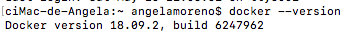
\includegraphics[width=8cm,height=8cm,keepaspectratio]{./Contenedores/Azure/10.png}
\end{nscenter}
\newline
A continuación voy a desplegar un contenedor a partir de unas imágenes de un 
repositorio en github que ofrece una aplicación de votos online. Para ello, 
clonamos el repositorio.
\newline
\begin{nscenter}
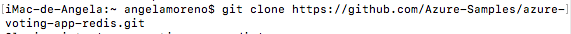
\includegraphics[width=8cm,height=8cm,keepaspectratio]{./Contenedores/Azure/11.png}
\end{nscenter}
\newline
A continuación, mostramos los contenedores que hay en ejecución.
\newline
\begin{nscenter}
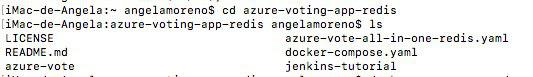
\includegraphics[width=8cm,height=8cm,keepaspectratio]{./Contenedores/Azure/12.png}
\end{nscenter}
\newline
El front de la aplicación está corriendo en localhost, en el puerto 8080. Por 
tanto, si vamos al explorador e intentamos acceder al puerto 8080 del localhost 
debería de aparecer la aplicación:
\newline
\begin{nscenter}
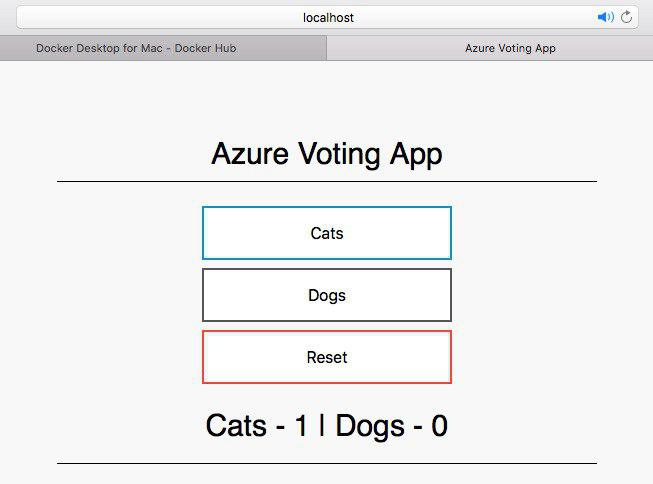
\includegraphics[width=8cm,height=8cm,keepaspectratio]{./Contenedores/Azure/13.png}
\end{nscenter}
\newline
A continuación, voy a mostrar de nuevo los contenedores que hay en ejecución:
\newline
\begin{nscenter}
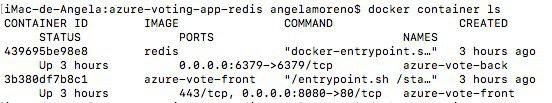
\includegraphics[width=8cm,height=8cm,keepaspectratio]{./Contenedores/Azure/14.png}
\end{nscenter}
\newline
Voy a intentar borrar uno de ellos, en concreto azure-vote-back:

\begin{nscenter}
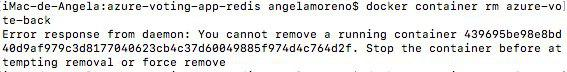
\includegraphics[width=8cm,height=8cm,keepaspectratio]{./Contenedores/Azure/15.jpg}
\end{nscenter}
\newline
Como se puede ver en la imagen, no deja borrar un contenedor que se esté 
ejecutando a no ser que lo paremos o que forcemos su borrado. Por tanto, fuerzo 
su borrado:
\newline
\begin{nscenter}
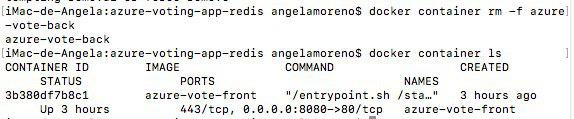
\includegraphics[width=8cm,height=8cm,keepaspectratio]{./Contenedores/Azure/16.jpg}
\end{nscenter}
\newline
Como se puede ver, el contenedor "azure-vote-back" ya no está activo, y si 
intentamos acceder de nuevo a la página donde está la aplicación nos vamos a 
encontrar con que ya no funciona:
\newline
\begin{nscenter}
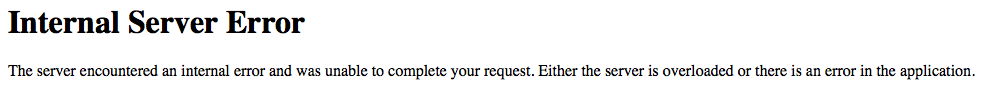
\includegraphics[width=8cm,height=8cm,keepaspectratio]{./Contenedores/Azure/17.png}
\end{nscenter}
\newpage
\subsection*{Creación de una aplicación en contenedores con Azure Web App for 
Containers}

App Service Linux proporciona pilas de aplicaciones predefinidas en Linux con 
compatibilidad con .NET, PHP y Node.js entre otros. En el ejemplo que viene a 
continuación se va a crear una web e implementar una imagen de GO desde Docker 
Hub. Para ello, voy a utilizar la CLI de Azure.

\subsubsection*{Crear un grupo de recursos}
Un grupo de recursos es un contenedor lógico en el que se implementan y 
administran recursos de Azure como aplicaciones web, bases de datos y cuentas de
almacenamiento. \\
Para crear dicho grupo de recursos, en la CLI de Azure, se introduce la 
siguiente instrucción: \\
\begin{nscenter}
\noindent\rule{10cm}{0.4pt}

az group create --name miGru --location "West Europe"

\noindent\rule{10cm}{0.4pt}
\end{nscenter}
\newline
El grupo creado se llama "miGru" y tiene como localización el oeste de Europa.\\
Como respuesta a la instrucción ejecutada la CLI de Azure mostrará un JSON donde
hará saber que la instrucción ha sido ejecutada correctamente y se ha creado el 
grupo.
\newline
\begin{nscenter}
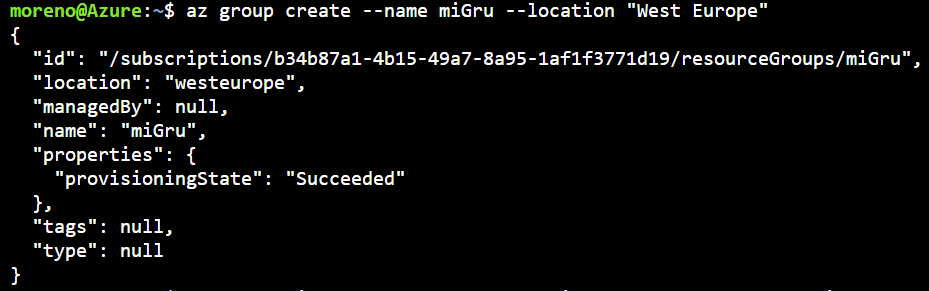
\includegraphics[width=8cm,height=8cm,keepaspectratio]{./Contenedores/Azure/2.png}
\end{nscenter}
\subsubsection*{Crear un plan de Azure App Service}
Se crea un plan App Service a través de la CLI de Azure:
\begin{nscenter}
\noindent\rule{10cm}{0.4pt}

az appservice plan create --name miPlan \\--resource-group miGru --ski B1 --is-linux

\noindent\rule{10cm}{0.4pt}
\end{nscenter}
\newline
El plan creado se llama miPlan y pertenece al grupo creado anteriormente.\\
Con el valor "B1" asignamos un plan de tarifa básico y con "--is-linux" 
determinamos que es un contenedor Linux.
\newline
\begin{nscenter}
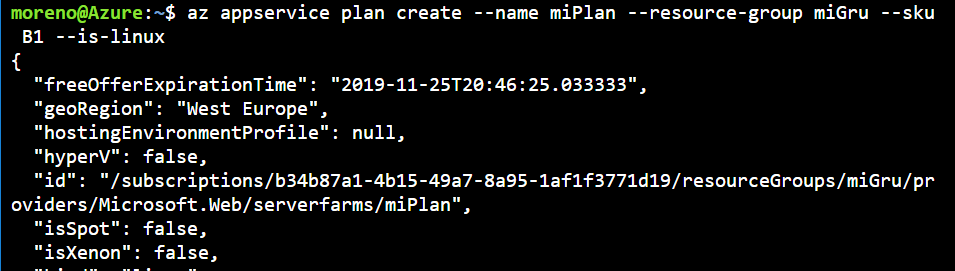
\includegraphics[width=8cm,height=8cm,keepaspectratio]{./Contenedores/Azure/3.png}
\end{nscenter}
\subsubsection*{Creación de una aplicación web}
Ahora, a través de la CLI, se va a crear una aplicación web.
\newline
\begin{nscenter}
\noindent\rule{10cm}{0.4pt}

az webapp create --resource-group miGru --plan miPlan --name nombreApplication 
--deployment-container-image-name microsoft/azure-appservices-go-quickstart

\noindent\rule{10cm}{0.4pt}
\end{nscenter}
\newline
Con el comando "--deployment-container-image-name" apuntamos a la imagen pública
de Docker Hub. \\
\begin{nscenter}
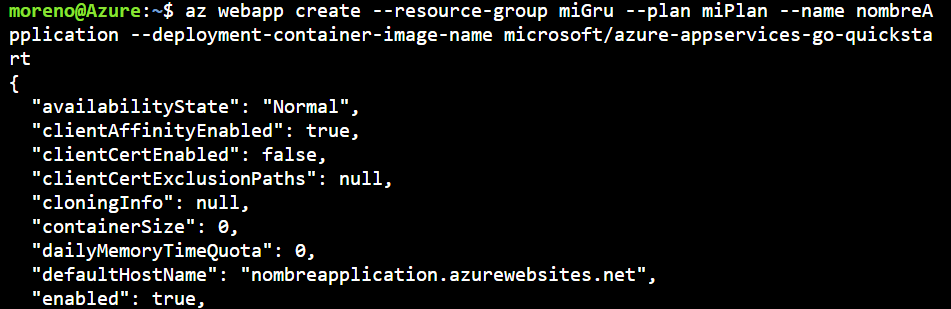
\includegraphics[width=8cm,height=8cm,keepaspectratio]{./Contenedores/Azure/4.png}
\end{nscenter}
\subsubsection*{Navegación hasta la aplicación}
Debido a que el nombre elegido pata el nombre de la aplicación web es 
"nombreApplication", la URL que deberemos de introducir en el navegador para ir 
a nuestra página web es la siguiente:\\
\begin{nscenter}
\noindent\rule{10cm}{0.4pt}

http:nombreapplication.azurewebsites.net/hello

\noindent\rule{10cm}{0.4pt}
\newline
\end{nscenter}
Mostrándose en el navegador lo siguiente:
\newline
\begin{nscenter}
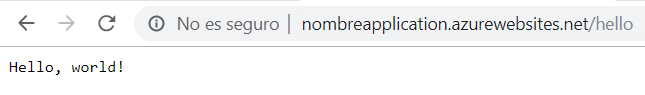
\includegraphics[width=8cm,height=8cm,keepaspectratio]{./Contenedores/Azure/5.png}
\end{nscenter}
\newpage
\subsection*{Ejecución a petición de aplicaciones de contenedor en Azure 
Container Instances}

En este apartado se va a usar la CLI de Azure para implementar un contenedor de 
docker aislado y hacer que la aplicación esté disponible con un nombre de 
dominio completo.\\
\subsubsection*{Creación de un grupo de recursos}
\begin{nscenter}
\noindent\rule{10cm}{0.4pt}

az group create --name myGroup --location "west Europe"

\noindent\rule{10cm}{0.4pt}
\end{nscenter}
\subsubsection*{Creación de un contenedor}
Para crear una instancia de contenedor de la CLI de Azure hay que proporcionar 
un nombre al grupo de recursos, un nombre de instancia de contenedor y una 
imagen de contenedor de Docker. En este ejemplo se usa una pública, que 
empaqueta una aplicación en Node.js que sirve una página HTML estática.\\
Los contenedores se pueden exponer en Internet mediante la especificación para 
que se abran uno o varios puertos.\\
Mediante la etiqueta "--dnd-name-label" se le establece un valor DNS.
\begin{nscenter}
\noindent\rule{10cm}{0.4pt}

az container create --resource-group myGroup --name mycontainer 
--image mcr.microsoft.com/azuredocs/aci-helloworld\\ --dns-name-label acidemo 
--ports 80

\noindent\rule{10cm}{0.4pt}
\end{nscenter}
\newline
A continuación, comprobamos el estado:
\newline
\begin{nscenter}
\noindent\rule{10cm}{0.4pt}

az container show --resource-group myGroup --name mycontainer\\ --query 
"{FQDN:ipAddress.fqdn,ProvisioningState:provisioningState}" --out table
\noindent\rule{10cm}{0.4pt}
\end{nscenter}
\newline
\begin{nscenter}
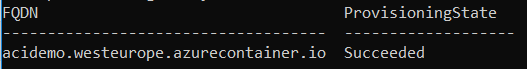
\includegraphics[width=8cm,height=8cm,keepaspectratio]{./Contenedores/Azure/6.png}
\end{nscenter}

El estado es "Succeeded", por lo que sí introducimos el FQDN en el navegador, 
lo que se muestra es lo siguiente:
\newline
\begin{nscenter}
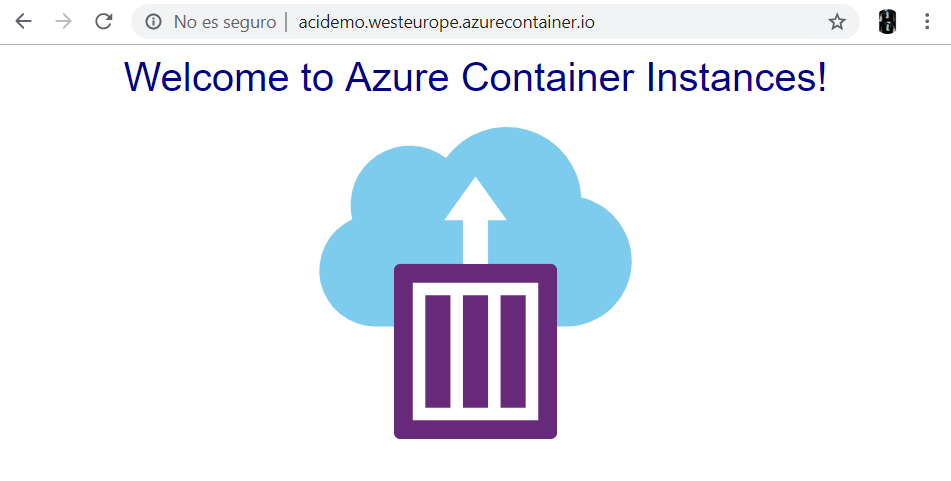
\includegraphics[width=8cm,height=8cm,keepaspectratio]{./Contenedores/Azure/7.png}
\end{nscenter}

\subsubsection*{Extraer los registros del contenedor}

\begin{nscenter}
\noindent\rule{10cm}{0.4pt}

az container logs --resource-group myGroup --name mycontainer

\noindent\rule{10cm}{0.4pt}
\end{nscenter}
\newline
\begin{nscenter}
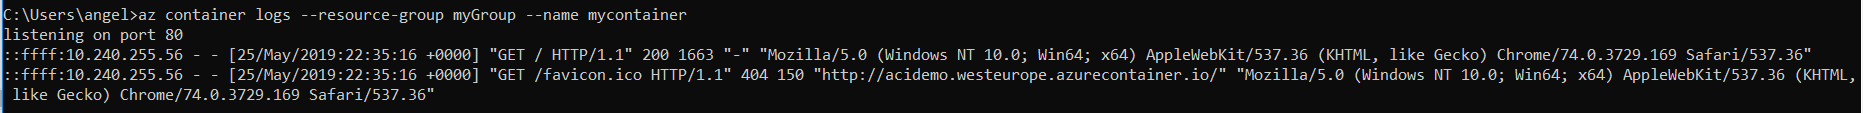
\includegraphics[width=12cm,height=12cm,keepaspectratio]{./Contenedores/Azure/8.png}
\end{nscenter}
\newline
Se muestran los registros del contenedor, addemás de las solicitudes HTTP GET 
generadas al ver la aplicación en el explorador.
\newpage
\subsection*{Creación de un registro de Docker privado en Azure Container Registry}

Para esta subsección, al contrario que en todas las anteriores desarrolladas, he
tenido que instalarme la CLI de Azure, no pudiendo utilizar la versión Cloud.

\subsubsection*{Crear un grupo de recursos}
\begin{nscenter}
\noindent\rule{10cm}{0.4pt}

az group create --name miGrupo --location "West Europe"

\noindent\rule{10cm}{0.4pt}
\end{nscenter}

\subsubsection*{Crear un registro de contenedor}
\begin{nscenter}
\noindent\rule{10cm}{0.4pt}

az acr create --resource-group miGrupo --name miRegistro0024 --sku Basic

\noindent\rule{10cm}{0.4pt}
\end{nscenter}

\subsubsection*{Insertar la imagen en el registro}
\begin{nscenter}


\noindent\rule{10cm}{0.4pt}

az acr login --name miRegistro0024

\noindent\rule{10cm}{0.4pt}
\end{nscenter}

En este paso, sin embargo, se muestra lo siguiente por la CLI:
\newline
\begin{nscenter}
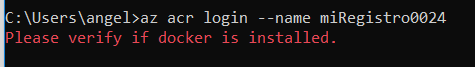
\includegraphics[width=8cm,height=8cm,keepaspectratio]{./Contenedores/Azure/9.png}
\end{nscenter}
\newline
Tal y como se puede ver, no se puede seguir adelante sin tener Docker instalado.
\\ El problema en este caso es que, al intentar instalar Docker una de las 
restricciones es que se debe de tener Windows 10 Pro, el cual yo no tengo. \\
Por tanto, se va a repetir todo el proceso desde el ordenador cuyo sistema 
operativo es macOS Sierra y donde sí que pude instalar Docker. \\
Antes de insertar imágenes hay que iniciar sesión en la instancia de Azure 
container Registry especificando el nombre del contenedor creado. En mi caso, 
y debido al cambio de ordenador, el nuevo nombre del registro es 
'registromoreno'. \\ También ejecuto un 'az acr show' para obtener el nombre del
servidor de inicio de sesión completo de la instancia de Azure Container 
Registry.
\newline
\begin{nscenter}
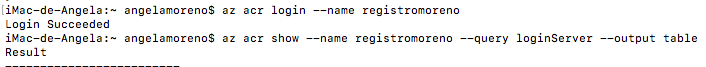
\includegraphics[width=8cm,height=8cm,keepaspectratio]{./Contenedores/Azure/51.png}
\end{nscenter}
\newline
A continuación se muestra la lista de imágenes locales con el comando 'docker 
images' y podemos que aparece 'aci-tutorial-app', que es la imagen creada en 
apartados anteriores.
\newline
\begin{nscenter}
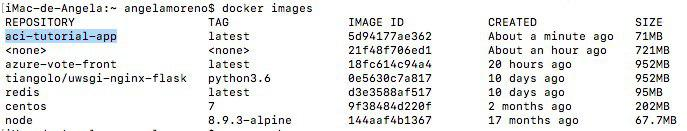
\includegraphics[width=8cm,height=8cm,keepaspectratio]{./Contenedores/Azure/18.jpg}
\end{nscenter}
\newline
Como siguiente paso etiquetamos la imagen aci-tutorial-app.
\newline
\begin{nscenter}
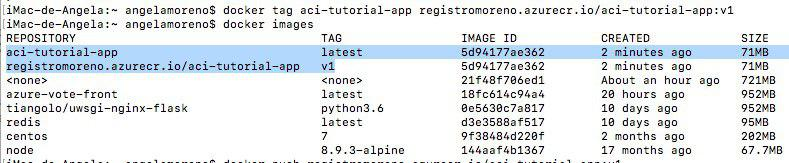
\includegraphics[width=8cm,height=8cm,keepaspectratio]{./Contenedores/Azure/19.jpg}
\end{nscenter}
\subsubsection*{Inserción de imágenes en Azure Container Registry}
Ahora que se ha etiquetado la imagen con el nombre del servidor de inicio de 
sesión completo, se puede insertar en el registro con el comando 'docker push'.
\newline
\begin{nscenter}
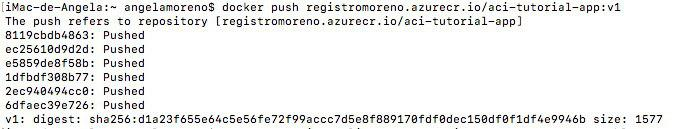
\includegraphics[width=8cm,height=8cm,keepaspectratio]{./Contenedores/Azure/20.jpg}
\end{nscenter}
\subsubsection*{Lista de imágenes en Azure Container Registry}
Ahora ejecuto el comando 'az acr repository list' para ver si la imagen se ha 
insertado correctamente. Y por último, con el comando 'az acr repository 
show-tags' hago que se imprima la etiqueta de la imagen.
\newline
\begin{nscenter}
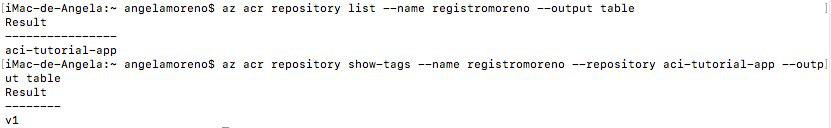
\includegraphics[width=8cm,height=8cm,keepaspectratio]{./Contenedores/Azure/21.jpg}
\end{nscenter}
\newpage
\section*{AWS}
Con respecto a AWS, los casos de uso de los contenedores son: microservicios, 
para aislar procesos; procesamiento de lotes, para arrancarlos con rapidez y 
escalarlos de forma dinámica dependiendo de la demanda; aplicaciones híbridas, 
puesto que los contenedores le permiten administrar de un modo uniforme la forma
en que se implementa el código y la migración de aplicaciones a la nube, puesto 
que los contenedores facilitan la tarea de empaquetar aplicaciones enteras y 
trasladarlas a la nube sin cambiar nada del código. También permiten diseñar 
plataformas para que los desarrolladores no tengan que administrar 
infraestructuras y aprendizaje automático. A su vez, Amazon tiene diferentes 
servicios: Amazon ECR, Amazon ECS, Amazon EKS, AWS Fargate y Amazon EC2.


\newpage
\subsection*{Amazon ECR}
Servicio para almacenar imágenes en contenedores. Los desarrolladores pueden 
usar la CLI de Docker para diseñar, insertar, extraer y administrar imágenes.

\subsubsection*{Componentes}
Registro: Cada cuenta de AWS recibe un registro de Amazon ECR donde puede crear 
repositorios de imágenes y guardar imágenes en ellos.\\
Token de autorización: Debe autenticar el cliente de Docker en los registros de 
Amazon ECR cono usuario de AWS para que dicho cliente pueda insertar y extraer 
imágenes. A través del comando get-login de la AWS CLI se proporcionan 
credenciales para pasarlas al Docker.\\
Repositorio: Contiene las imágenes de Docker.\\
Política sobre repositorios: Se puede controlar el acceso a los repositorios e 
imágenes. \\
Imagen: Se puede insertar y extraer imágenes de Docker en los repositorios y 
usarlas localmente.
\subsubsection*{Introducción a Amazon ECR}
En este apartado nos van a enseñar a crear un repositorio en la consola de 
Amazon ECR. Para ello, abro la consola de Amazon ECR y selecciono el nombre que 
va a tener el primer repositorio, que va a ser angelamoreno. \\
Una vez introducido el nombre y creado el repositorio, AWS muestra la siguiente 
interfaz:
\newline
\begin{nscenter}
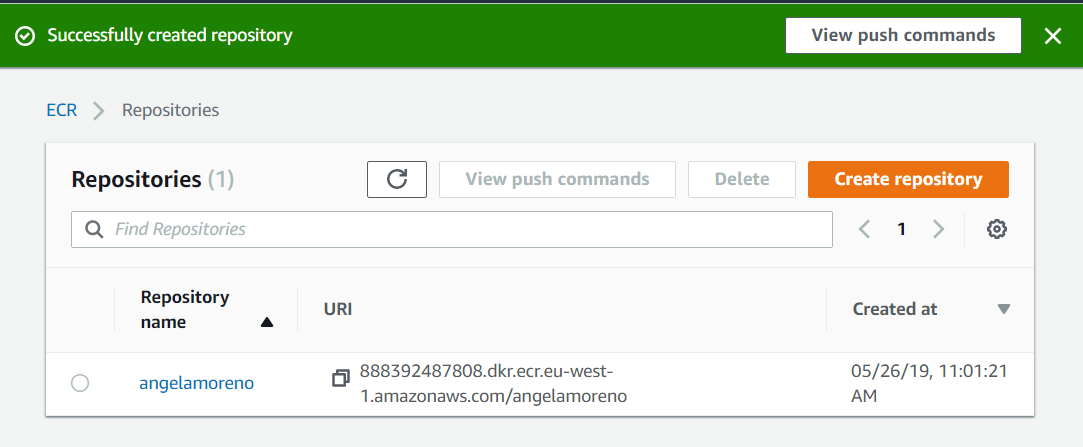
\includegraphics[width=8cm,height=8cm,keepaspectratio]{./Contenedores/AWS/27.png}
\end{nscenter}
\subsubsection*{Creación, etiquetado y envío de imágenes Docker}
Lo primero que hay que hacer es instalar la CLI de AWS. Una vez hecho, 
ejecutamos el comando 'aws configure'. \\
Al ejecutar el comando 'aws configure' nos va a pedir que introduzcamos una 
clave de acceso ID, una contraseña de acceso, el nombre de la región en la que 
se creó el repositorio y el tipo de output por defecto. \\
Para obtener el ID y la contraseña hay que ir al IAM Management Console de AWS, 
al apartado de Usuarios y generar una clave de acceso. El ID y la contraseña 
generadas en el momento son las que tenemos que introducir en la CLI de AWS. \\
A continuación, ejecutando el comando 'docker login' se pedirán los credenciales
de Docker. \\
\newline
\begin{nscenter}
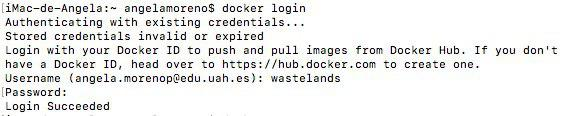
\includegraphics[width=8cm,height=8cm,keepaspectratio]{./Contenedores/AWS/17.jpg}
\end{nscenter}
\newline
A partir de ese momento, a través de los comandos 'docker tag' y 'docker push' 
podremos insertar imágenes en el repositorio creado.

\newpage
\subsection*{Introducción a Amazon ECS}
Amazon Elastic Container (Amazon ECS) es un servicio de administración de 
contenedores muy escalable y rápido que facilita la tarea de ejecutar, detener 
y gestionar contenedores de Docker en un clúster de instancias de Amazon EC2.\\
Para configurar un ECS hay que seguir los siguientes pasos: \\
Primero creamos una cuenta de AWS en http://aws.amazon.com/ y después darnos a 
nosotros mismos el permiso de ser administradores.
\begin{nscenter}
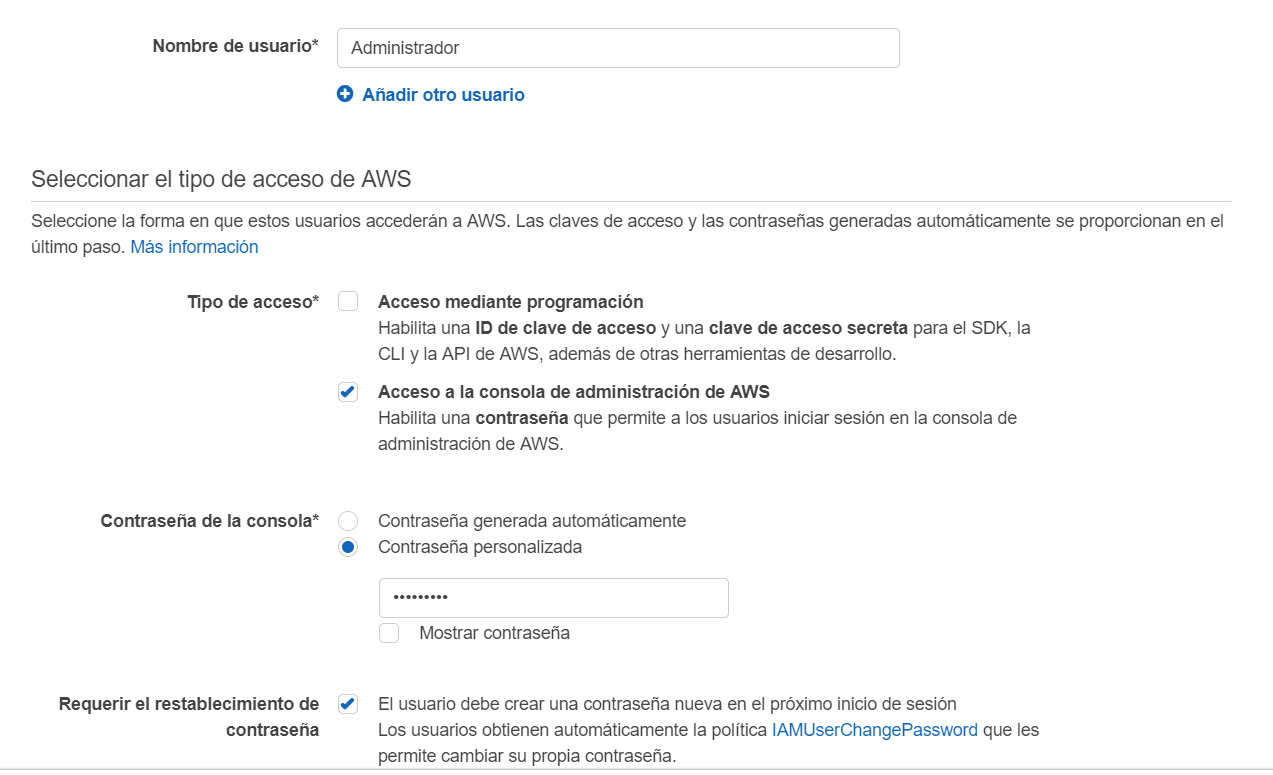
\includegraphics[width=8cm,height=8cm,keepaspectratio]{./Contenedores/AWS/28.png}
\end{nscenter}
\newline
A continuación hay que crear un grupo, el cual va a tener de nombre 
Administrators donde, al usuario previamente creado, se le asignan unas 
políticas. \\
Una vez asignadas y creado el usuario, la pantalla es la siguiente: 
\newline
\begin{nscenter}
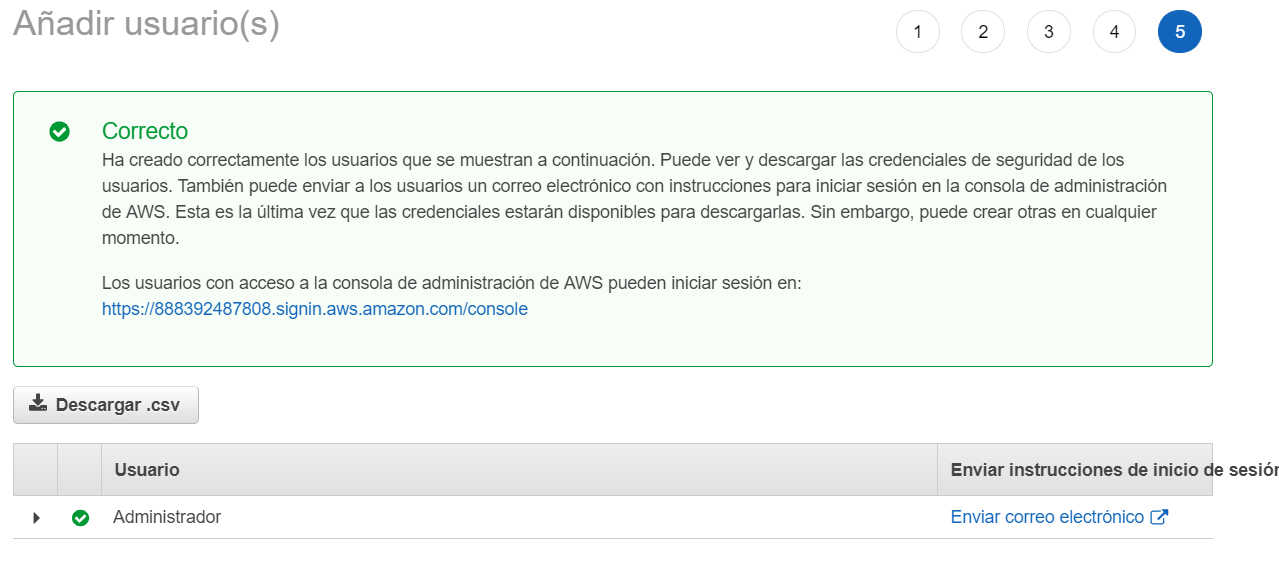
\includegraphics[width=8cm,height=8cm,keepaspectratio]{./Contenedores/AWS/29.png}
\end{nscenter}
\newline
Una vez creado el usuario, nos piden que accedamos a él.
\newline
\begin{nscenter}
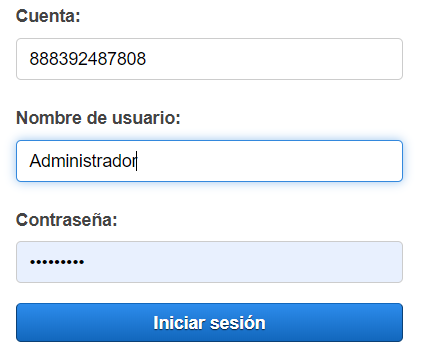
\includegraphics[width=8cm,height=8cm,keepaspectratio]{./Contenedores/AWS/30.png}
\end{nscenter}
\newline
Tal y como se seleccionó en las opciones al crear el usuario, al iniciar sesión,
el administrador tiene que cambiar la contraseña antigua por una nueva.\newline
\newline
\begin{nscenter}
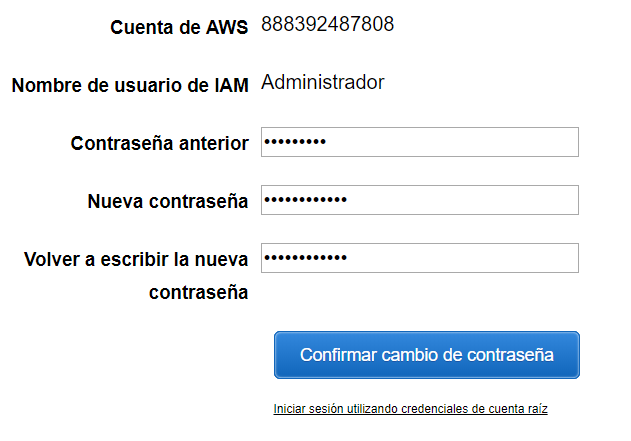
\includegraphics[width=8cm,height=8cm,keepaspectratio]{./Contenedores/AWS/31.png}
\end{nscenter}
\newline
Después de esto, ya podemos crear una VPC (nube virtual privada). \\
Para ello, lo que hay que hacer es abrir la consola de Amazon VPC y lanzar el 
asistente de VPC, la cual tenga una única subred pública. También hay que 
ponerle un nombre, el cual va a ser angelamoreno. Una vez que se ha creado, la 
pantalla que nos muestra AWS es la siguiente: 
\newline
\begin{nscenter}
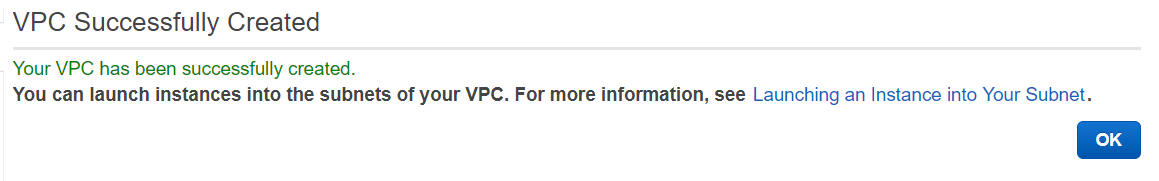
\includegraphics[width=8cm,height=8cm,keepaspectratio]{./Contenedores/AWS/32.png}
\end{nscenter}
\newline
\newpage
\subsection*{Introducción a Amazon EKS}
Amazon Elastic Container Service for Kubernetes (Amazon EKS) es un servicio 
administrado que permite ejecutar Kubernetes AWS sin necesidad de crear ni 
mantener su propio plano de control de Kubernetes. Kubernetes es un sistema de 
código abierto para automatizar la implementación, escalado y administración de 
las aplicaciones en contenedores. \\
Amazon EKS detecta y reemplaza automáticamente las instancias del plano de 
control en mal estado, y proporciona actualizaciones de versiones y parches 
automatizados para ellas. También integra numerosos servicios AWS para ofrecer 
escalabilidad y seguridad a las aplicaciones, como IAM para la autenticación, 
Amazon VPC para el aislamiento...
\subsubsection*{Creación del clúster de Amazon EKS y los nodos de trabajo}
Para hacer esta parte de la práctica he tenido que instalar eksctl y kubectl. \\
Inicialmente creamos el clúster de Amazon EKS y los nodos de trabajo con el 
siguiente comando:
\newline
\begin{nscenter}
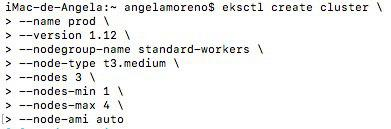
\includegraphics[width=8cm,height=8cm,keepaspectratio]{./Contenedores/AWS/22.jpg}
\end{nscenter}
\subsubsection*{Lanzar aplicación de libro de invitados}
Para lanzar la aplicación de libro de invitados hay que crear el controlador de 
replicación maestro Redis, además de crear el servicio, el controlador de 
replicación esclavo, el servicio esclavo Redis, también crear el controlador de 
replicación de guestbook y el servicio guestbook.
\newline
\begin{nscenter}
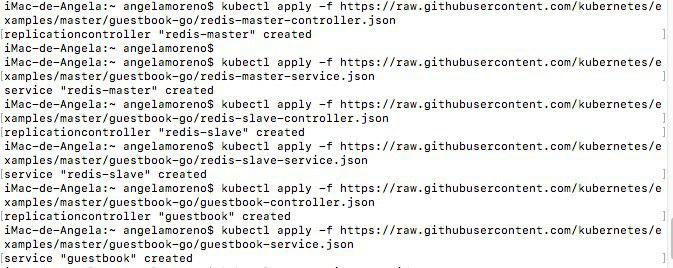
\includegraphics[width=8cm,height=8cm,keepaspectratio]{./Contenedores/AWS/23.jpg}
\end{nscenter}
\newline
Por último, hay que mirar la dirección externa del servicio guestbook a través 
del comando 'kubectl get services -o wide'.
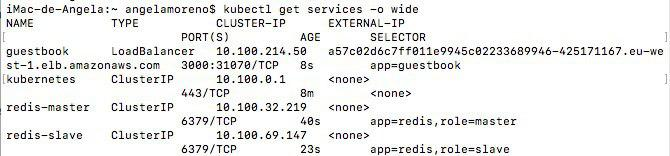
\includegraphics[width=8cm,height=8cm,keepaspectratio]{./Contenedores/AWS/2.jpg}
\subsubsection*{Uso de Heml con Amazon EKS}
Para esta parte de la práctica hay que crear, a través de la consola, un 
servidor y un cliente que se conecta a dicho servidor creado.
\newline
\begin{nscenter}
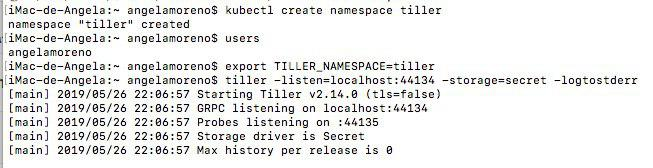
\includegraphics[width=8cm,height=8cm,keepaspectratio]{./Contenedores/AWS/24.jpg}
\end{nscenter}
\newline
En el terminal del servidor de tiller se establece la variable de entorno 
TILLER NAMESPACE y a continuación se inicia el servidor. \\
A continuación, en la terminal de cliente helm, establecemos la variable de 
entorno HELM HOST:44134 y nos conectamos al servidor.
\newline
\begin{nscenter}
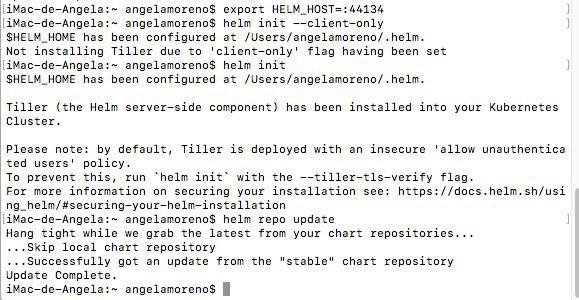
\includegraphics[width=8cm,height=8cm,keepaspectratio]{./Contenedores/AWS/25.jpg}
\end{nscenter}
\newpage
\subsection*{Introducción a Amazon EC2}
Amazon Elastic Compute Cloud (amazon EC2) proporciona capacidad de computación 
escalable en la nuble de Amazon Web Services (AWS) El uso de Amazon EC2 elimina 
la necesidad de invertir en hardware.
\subsubsection*{Lanzar una instancia}
Para crear una instancia hay que hacer uso de la consola de Amazon EC2. \\
Una vez que se ha seleccionado el lanzar una instancia, hay que elegir una 
imagen de máquina de Amazon (AMI), que en mi caso ha sido la Windows Server 
2016 Base, como se muestra a continuación. Ésta AMI está marcada como Free tier 
eligible.
\newline
\begin{nscenter}
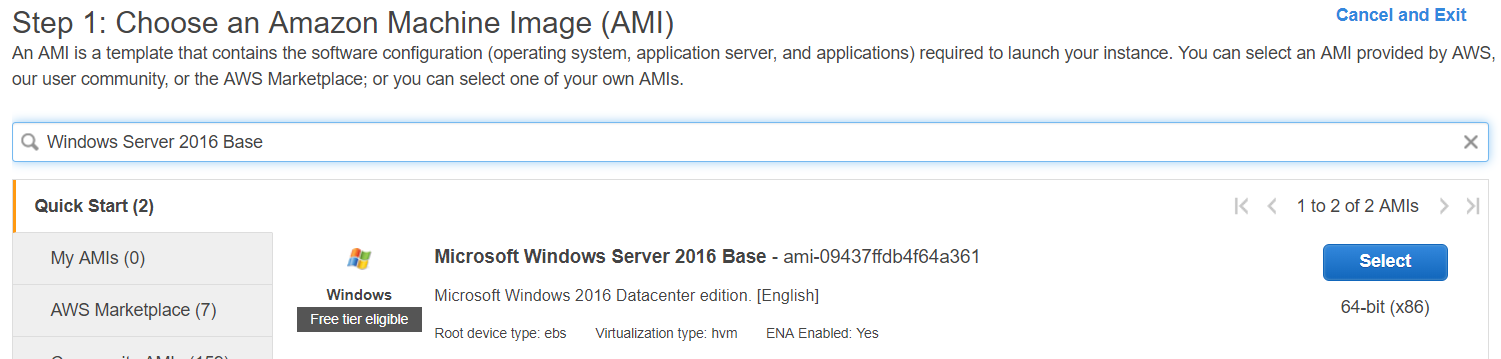
\includegraphics[width=8cm,height=8cm,keepaspectratio]{./Contenedores/AWS/33.png}
\end{nscenter}
\newline
A continuación hay que elegir un tipo de instancia, quedándonos con la t2.micro 
que es la que viee por defecto; después de esto, revisamos y lanzamos.
\newline
\begin{nscenter}
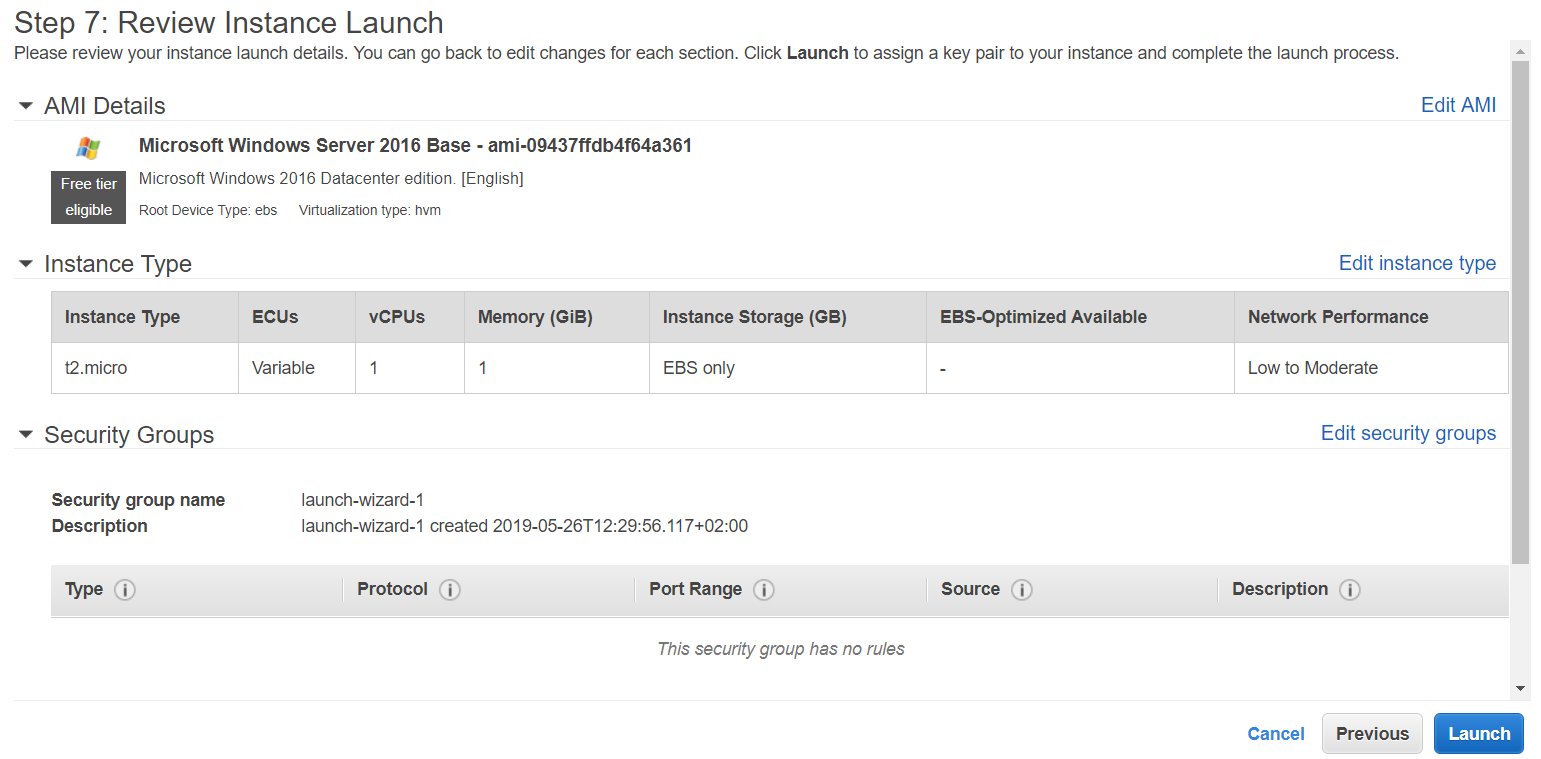
\includegraphics[width=8cm,height=8cm,keepaspectratio]{./Contenedores/AWS/34.png}
\end{nscenter}
\newline
Al ir a lanzar la instancia, nos hace descargarnos un par de llaves, a las 
cuales les tienes que asignar un nombre, siendo angelamorenokey el elegido. 
Descarga un archivo que se corresponde con esas llaves.
\newline
\begin{nscenter}
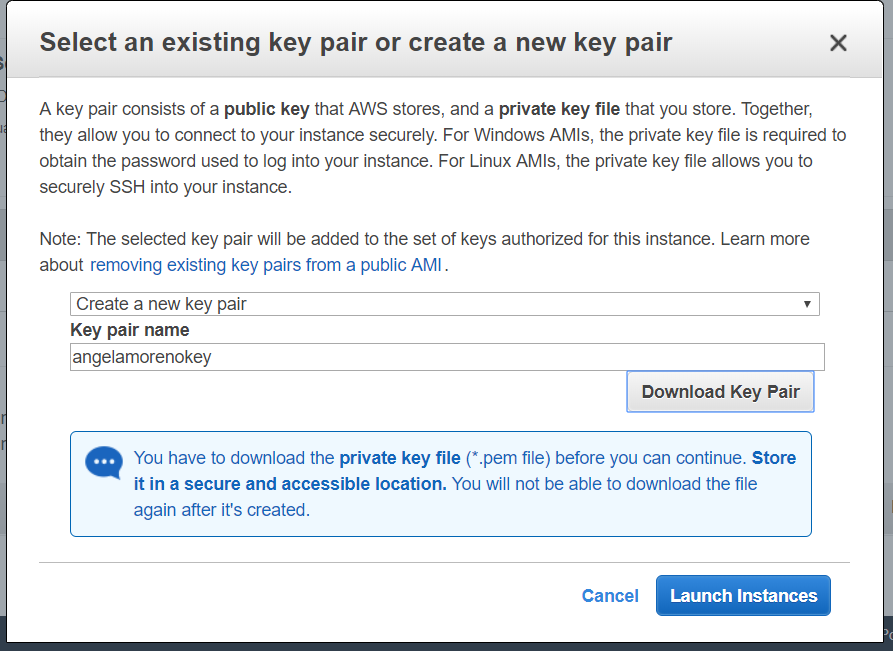
\includegraphics[width=8cm,height=8cm,keepaspectratio]{./Contenedores/AWS/35.png}
\end{nscenter}
\newline
Por último, si le damos a lanzar, la instancia queda lanzada y, a partir de ese 
momento, podemos conectarnos a ella.
\newline
\begin{nscenter}
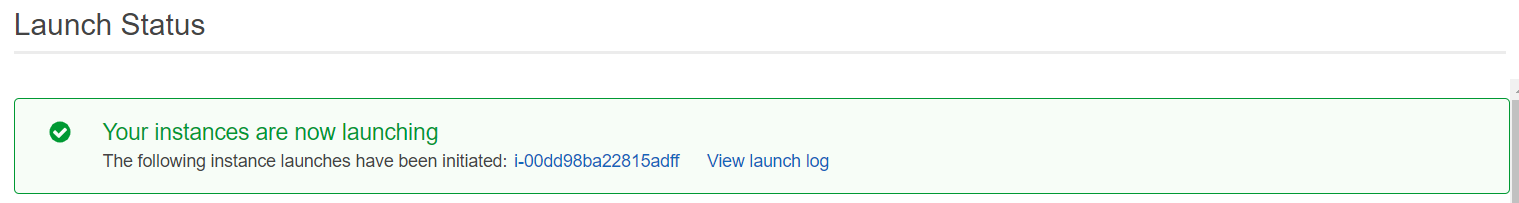
\includegraphics[width=8cm,height=8cm,keepaspectratio]{./Contenedores/AWS/36.png}
\end{nscenter}
\newline
\subsubsection*{Conectarnos a la instancia}

Para conectarnos a la instancia tenemos que volver a hacer uso de Amazon EC2, 
seleccionar la instancia creada anteriormente y conectarnos a ella.
\newline
\begin{nscenter}
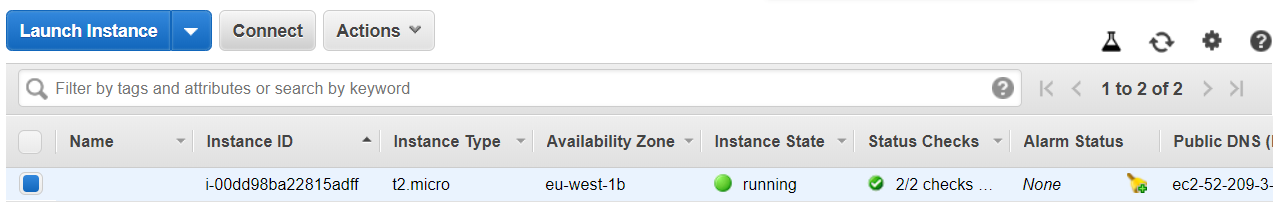
\includegraphics[width=8cm,height=8cm,keepaspectratio]{./Contenedores/AWS/37.png}
\end{nscenter}
\newline
Una vez que hayamos seleccionado el conectarnos a la instancia recién creada, 
AWS nos va a pedir que carguemos el archivo descargado previamente que contiene 
las dos llaves, el cual guardé bajo el nombre de angelamorenokey, que tiene 
formato .pem.
\newline
\begin{nscenter}
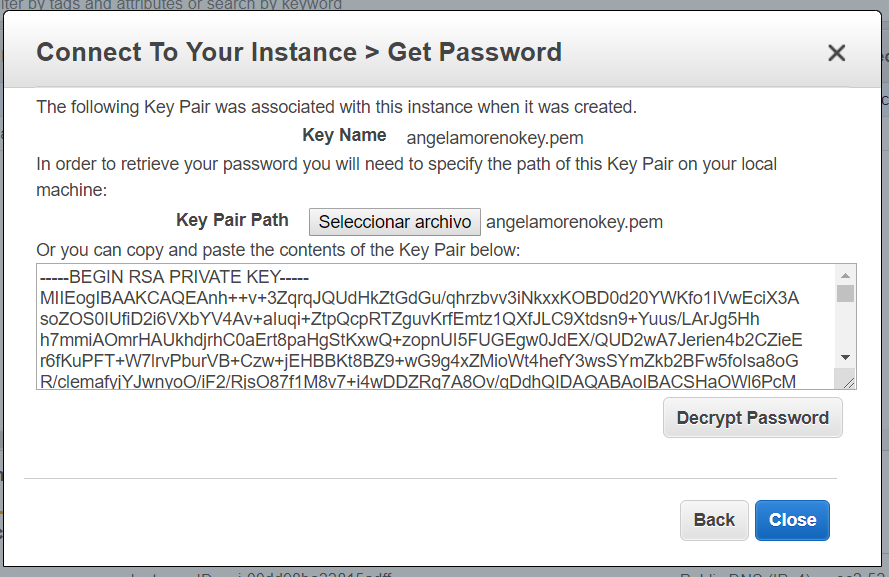
\includegraphics[width=8cm,height=8cm,keepaspectratio]{./Contenedores/AWS/38.png}
\end{nscenter}
\newline
Una vez cargado y al hacer click sobre 'Decrypt Password' podemos ver la 
contraseña generada resultante de subir dicho archivo .pem, correspondiente al 
usuario 'Administrador' que creamos anteriormente. 
\newline
\begin{nscenter}
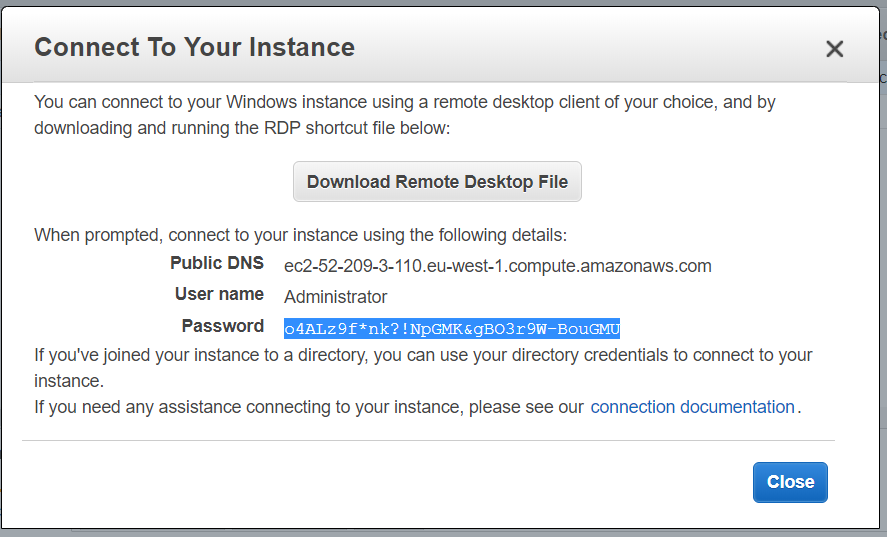
\includegraphics[width=8cm,height=8cm,keepaspectratio]{./Contenedores/AWS/39.png}
\end{nscenter}
\newline
Al hacer click sobre 'Download Remote Desktop File' se descarga un .rdp que, al 
ejecutarlo, va a permitir que nos conectemos a la instancia creada.
\newline
\begin{nscenter}
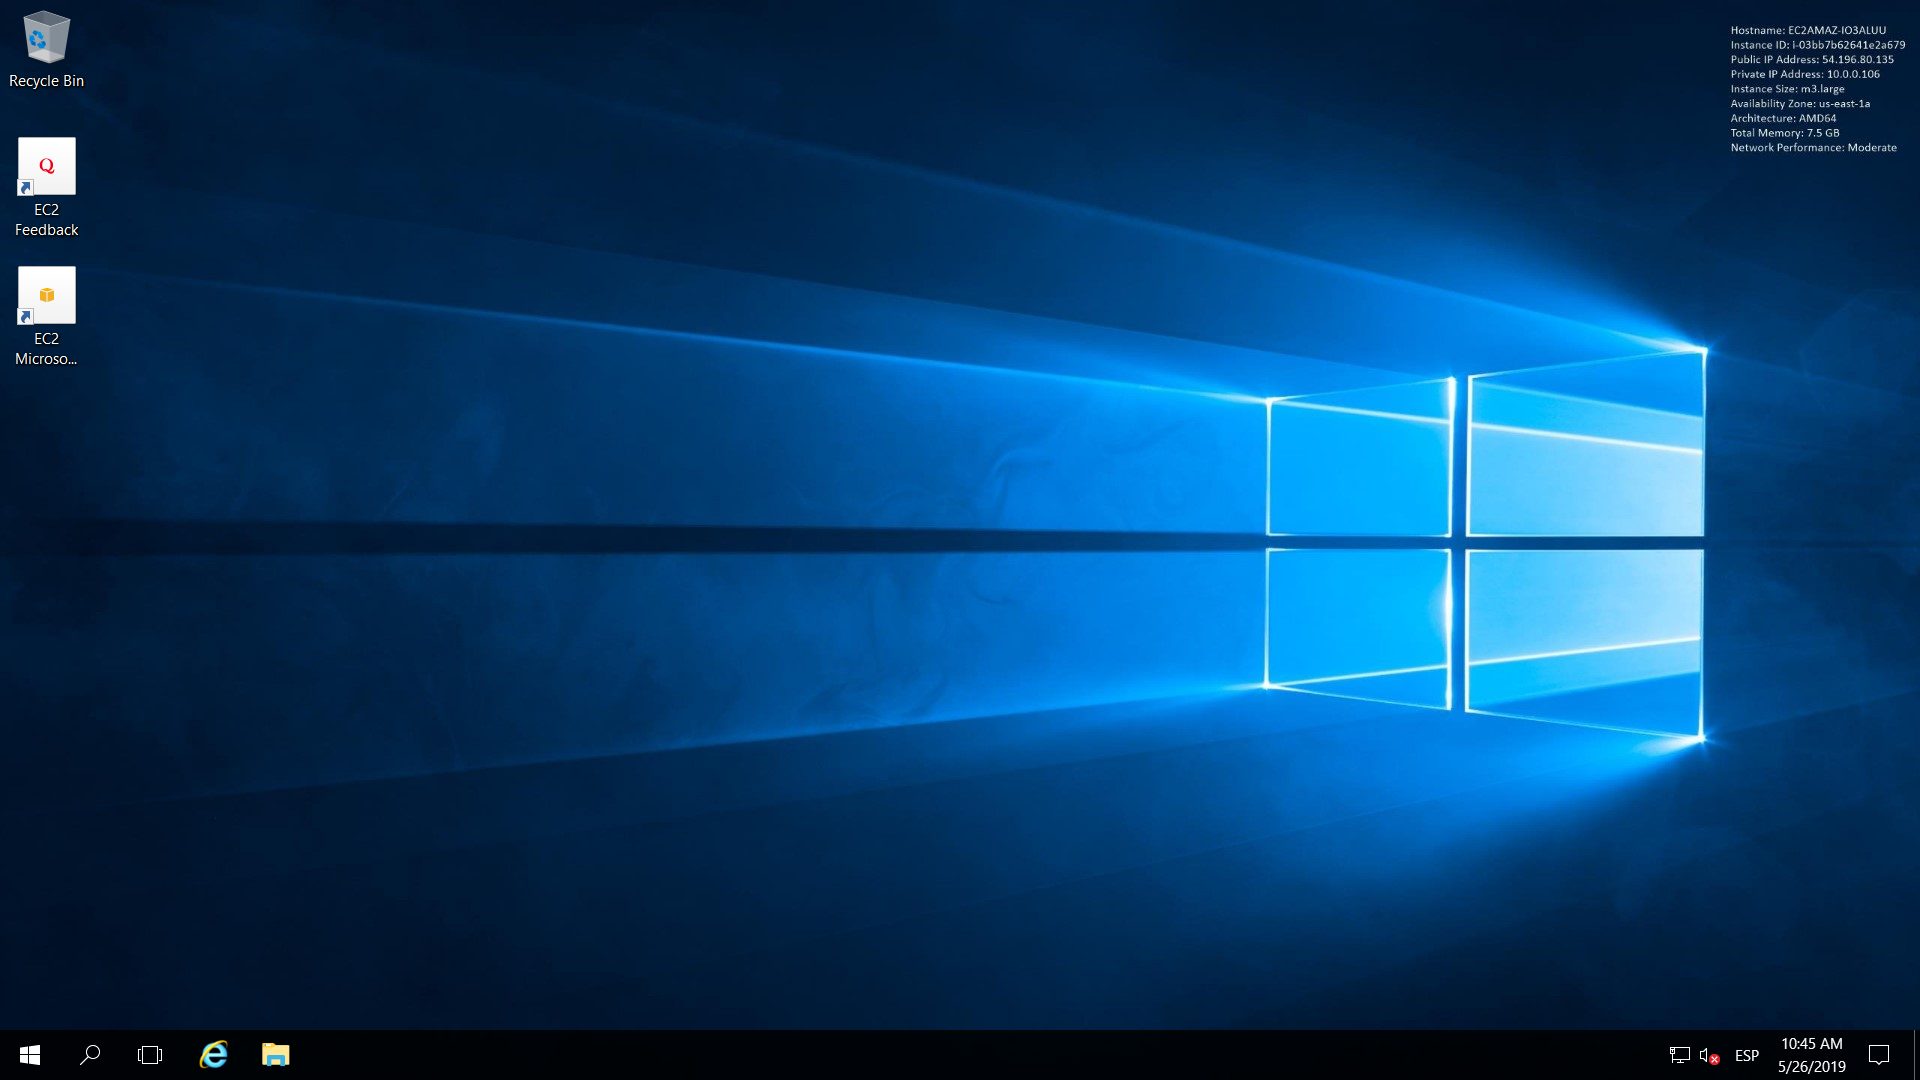
\includegraphics[width=8cm,height=8cm,keepaspectratio]{./Contenedores/AWS/41.png}
\end{nscenter}
\newline
Una vez que hayamos terminado con la instancia, tal y comos e indica en la guía 
proporcionada por AWS, hay que borrarla.
\newline
\begin{nscenter}
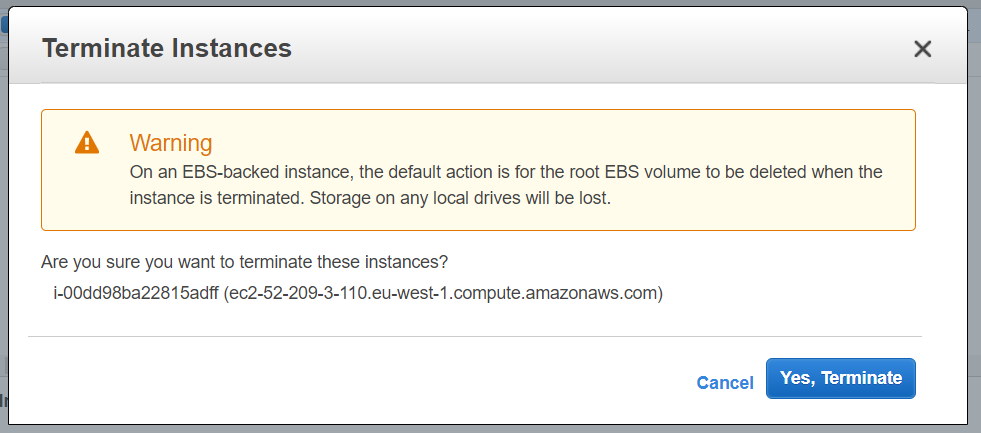
\includegraphics[width=8cm,height=8cm,keepaspectratio]{./Contenedores/AWS/42.png}
\end{nscenter}

\newpage
\subsection*{Implementar primer contenedor}
En este primer apartado, en AWS te permiten crear un primer contenedor.
\newline
\begin{nscenter}
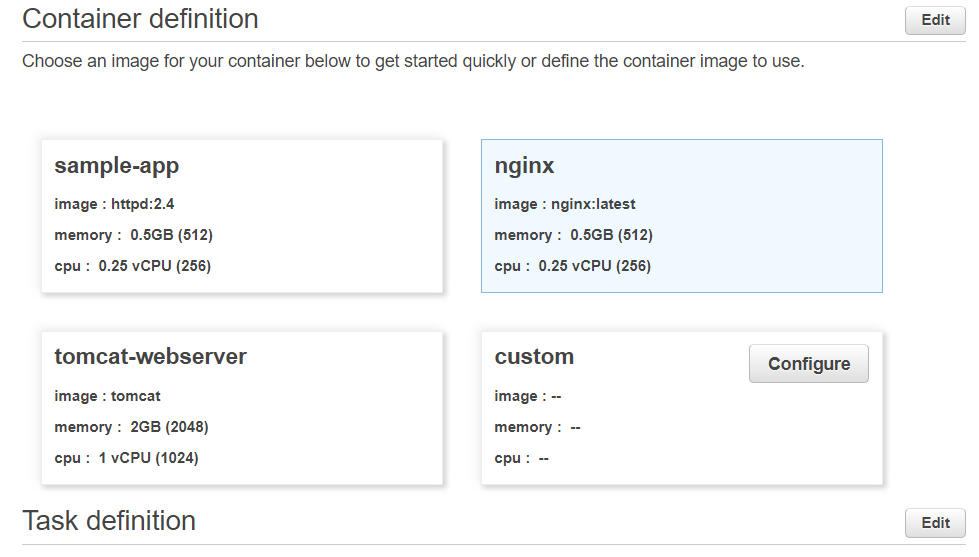
\includegraphics[width=8cm,height=8cm,keepaspectratio]{./Contenedores/AWS/18.png}
\end{nscenter}
\newline
También tienes que especificar el nombre del servicio y en qué puerto funcionará
, entre otros.\\ Una vez especificados las características de este primer 
contenedor, AWS lo crea.
\newline
\begin{nscenter}
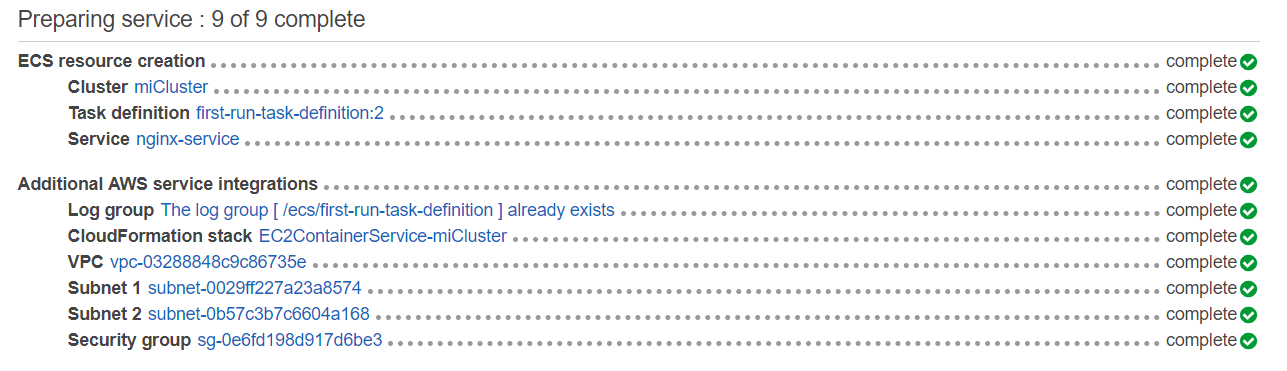
\includegraphics[width=8cm,height=8cm,keepaspectratio]{./Contenedores/AWS/19.png}
\end{nscenter}
\newline
\begin{nscenter}
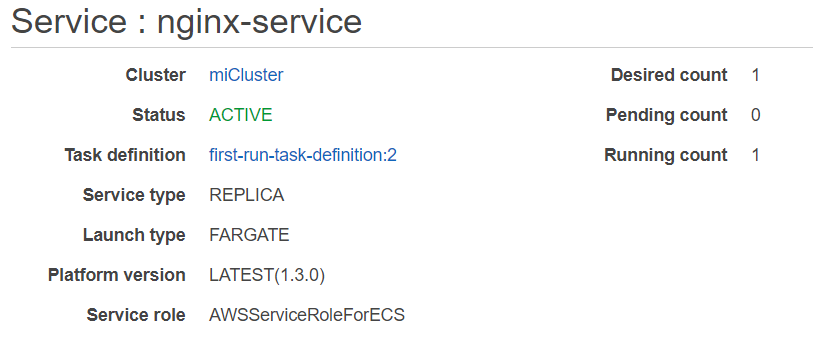
\includegraphics[width=8cm,height=8cm,keepaspectratio]{./Contenedores/AWS/20.png}
\end{nscenter}
\newpage
\subsection*{Crear una página web estática utilizando Amazon S3 y AWS Cloud 9}
Después de haber seleccionado mi localización, hay que acceder al servicio 
"Cloud9" desde la consola AWS, que es una nube para diseñar y depurar código.\\
Lo primero que hay que hacer, una vez hayamos accedido a la página que 
proporciona AWS de Cloud 9 es crear nuestro espacio de trabajo.
\newline
\begin{nscenter}
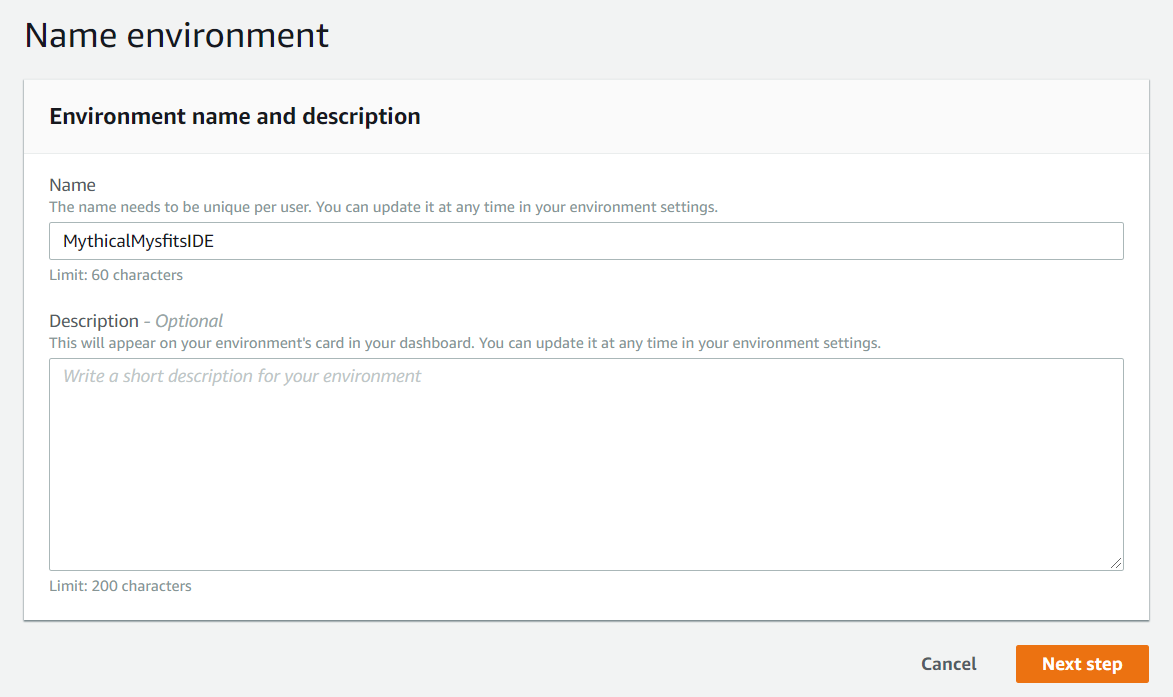
\includegraphics[width=8cm,height=8cm,keepaspectratio]{./Contenedores/AWS/21.png}
\end{nscenter}
\newline
Le he puesto "MythicalMysfitsIDE" como nombre al grupo de trabajo tal y como se 
muestra o indica en las instrucciones de AWS.
\newline
\begin{nscenter}
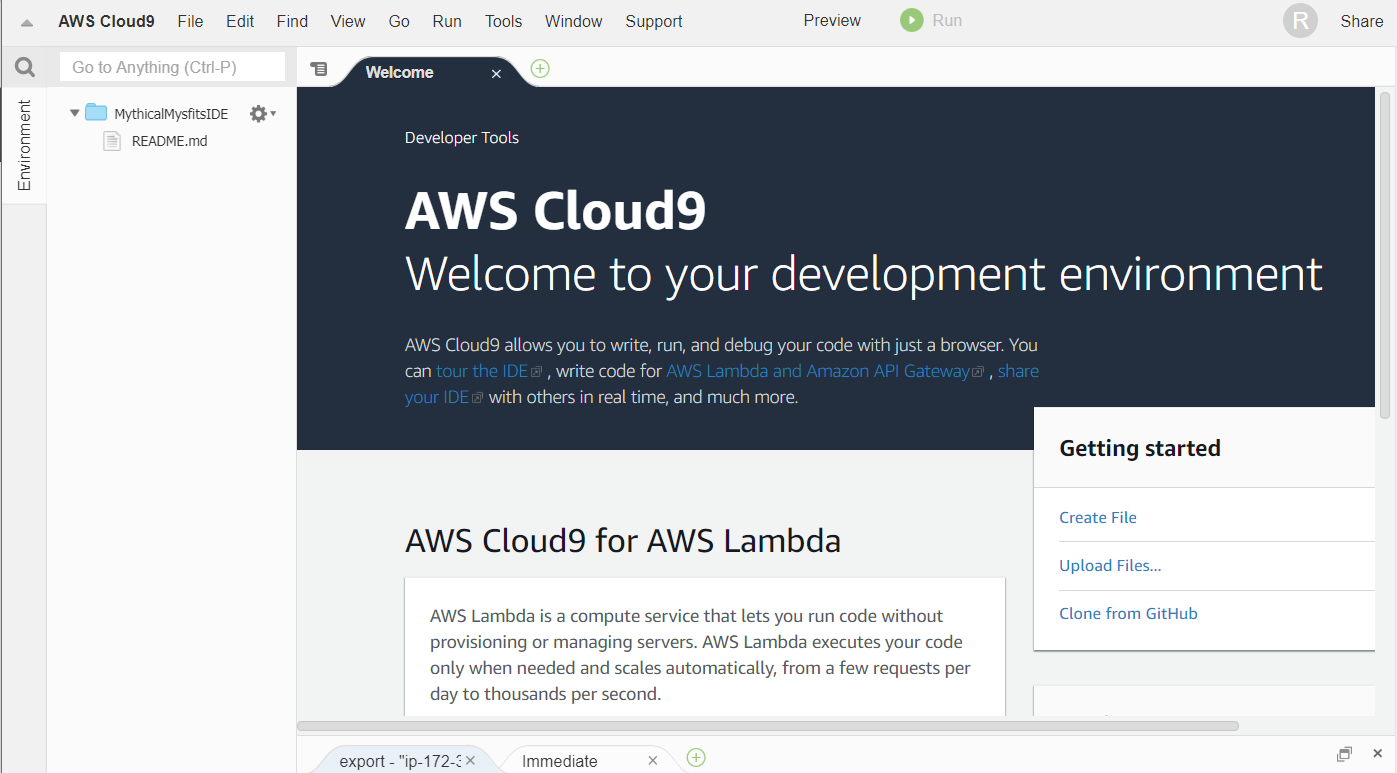
\includegraphics[width=8cm,height=8cm,keepaspectratio]{./Contenedores/AWS/22.png}
\end{nscenter}
\newline
Tal y como se muestra en la imagen, el espacio de trabajo se ha creado 
correctamente.\\ Piden inicialmente que clonemos el repositorio existente a 
través de la línea de comandos que está al final de la página previamente 
mostrada. Para ello, utilizo el siguiente comando:
\begin{nscenter}


\noindent\rule{10cm}{0.4pt}

git clone -b python https://github.com/aws-samples/aws-modern-application-workshop.git

\noindent\rule{10cm}{0.4pt}
\end{nscenter}

Una vez clonado, podemos ver que los archivos contenidos han cambiado.
\newline
\begin{nscenter}
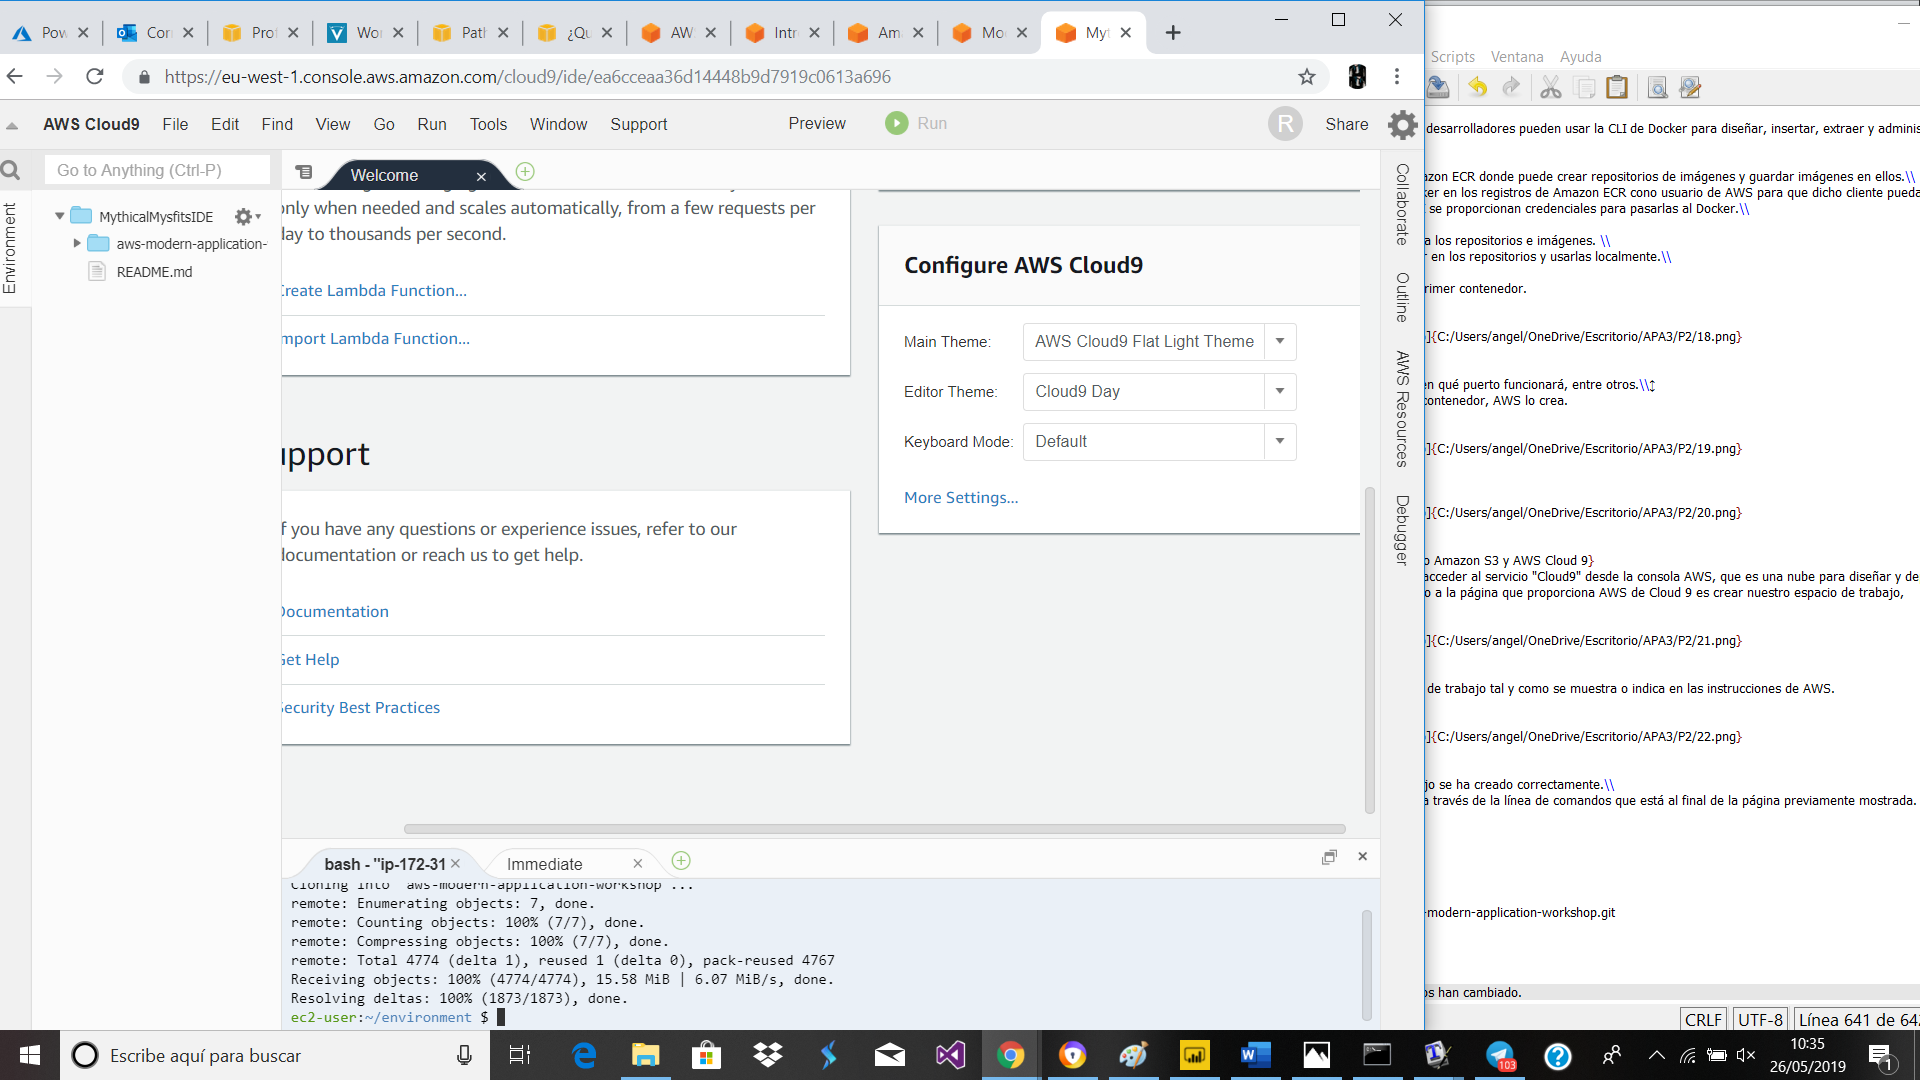
\includegraphics[width=8cm,height=8cm,keepaspectratio]{./Contenedores/AWS/23.png}
\end{nscenter}
\newline
A continuación, cambiamos de directorio.
\begin{nscenter}


\noindent\rule{10cm}{0.4pt}

cd aws-modern-application-workshop

\noindent\rule{10cm}{0.4pt}
\end{nscenter}

Siguiendo con este proceso, ahora toca creat la infaestructura donde se va a 
subir la página web que estamos creando.\\
Primero se va a crear un S3 bucket, y para ello hay que darle un nombre, 
siendo angelamoreno el nombre del bucket que yo he creado.\\
\begin{nscenter}


\noindent\rule{10cm}{0.4pt}

aws s3 mb s3://angelamoreno

\noindent\rule{10cm}{0.4pt}
\end{nscenter}
\newline
Ahora, una vez el bucket tenga nombre, vamos a configurarlo.
\begin{nscenter}


\noindent\rule{10cm}{0.4pt}

aws s3 website s3://angelamoreno --index-document index.html

\noindent\rule{10cm}{0.4pt}
\end{nscenter}
Por defecto, todos los buckets creados en AWS son privados, por lo que, para 
que puedan ser usados en una web pública, hay que cambiar la privacidad de 
dicho bucket, haciendo así que todos los objetos almacenados en él sean 
públicos para cualquiera. Esta configuración de la privacidad está localizada 
en un .json, el cuál tenemos que modificar. En concreto, el archivo que hay 
que modificar se llama "website-bucket-policy.json", al cuál se puede acceder a
través de los archivos del Cloud 9 anteriormente comentados.
\newline
\begin{nscenter}
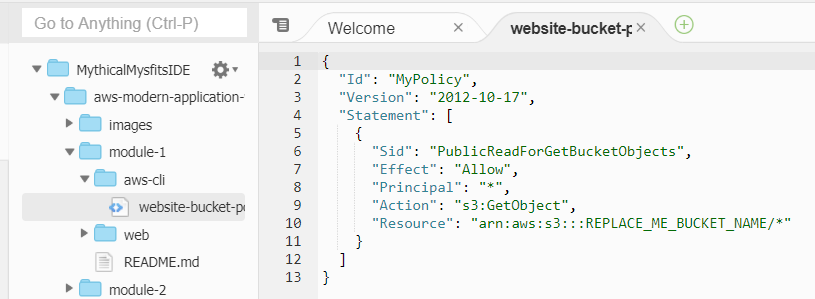
\includegraphics[width=8cm,height=8cm,keepaspectratio]{./Contenedores/AWS/24.png}
\end{nscenter}
\newline
\begin{nscenter}
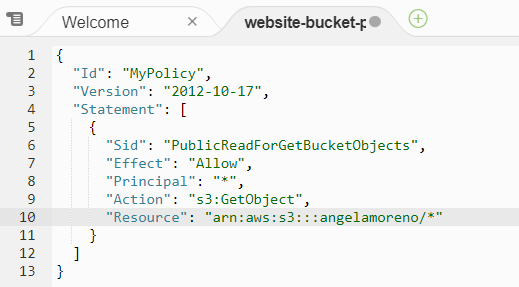
\includegraphics[width=8cm,height=8cm,keepaspectratio]{./Contenedores/AWS/25.png}
\end{nscenter}
\newline
A continuación, la siguiente instrucción se ha ejecutado a través de la CLI de 
AWS para terminar de configurar la privacidad del bucket.
\begin{nscenter}


\noindent\rule{10cm}{0.4pt}

aws s3api put-bucket-policy --bucket angelamoreno\\ 
--policy file://~/environment/aws-modern-application-workshop/module-1/aws-cli/website-bucket-policy.json

\noindent\rule{10cm}{0.4pt}
\end{nscenter}
\newline
A continuación, publicamos el contenido de la web en S3.
\begin{nscenter}
\noindent\rule{10cm}{0.4pt}
\newline
aws s3 cp\\ ~/environment/aws-modern-application-workshop/module-1/web/index.html\\ s3://angelamoreno/index.html
\noindent\rule{10cm}{0.4pt}
\end{nscenter}
\newline
Por último, una vez hecho esto, si vamos al navegador e introducimos la web que 
se detalla a continuación, tendremos acceso a la página web que hemos creado.
\begin{nscenter}
\noindent\rule{10cm}{0.4pt}
http://angelamoreno.s3-website-eu-west-1.amazonaws.com/
\noindent\rule{10cm}{0.4pt}
\end{nscenter}
Siendo angelamoreno el nombre del bucket y "eu-west-1" el código correspondiente
de localización de Irlanda (puesto que España no aparecía como posible 
localización).
\newline
\begin{nscenter}
\includegraphics[width=8cm,height=8cm,keepaspectratio]{./Contenedores/AWS/26.png}
\end{nscenter}
\newline

\newpage
\subsection*{Google Cloud}
Google Cloud utiliza la aplicación 'Container Engine' (GKE) para administrar y 
organizar clústeres que ejecuta contenedores Docker. Container Engine programa 
los contenedores en el clúster y los administra automáticamente en función de 
los requisitos definidos (como la CPU y la memoria). Está desarrollado en el 
sistema Kubernetes de código abierto, lo que permite aprovechar la 
infraestructura de la nube pública, híbrida o in situ.

\subsubsection*{Crear un clúster con GKE}

Lo primero que hay que hacer para poder crear un clúster es crear un proyecto; 
esto se hace a través de la página de Kubernetes Engine.
\newline
\begin{nscenter}
\includegraphics[width=8cm,height=8cm,keepaspectratio]{./Contenedores/Googlecloud/43.png}
\end{nscenter}
\newline
A continuación hay que elegir un shell, pudiendo usar la shell local o la shell 
proporcionada por Google Cloud, que es la que voy a usar yo. \\
Esta shell que viene dada por Google Cloud viene peinstalada con las 
herramientas de línea de comandos gcloud y kubectl; proporcionando la primera 
la interfaz de línea de comandos principal de GCP y la segunda la interfaz de 
línea de comandos para ejecutar los comandos en los clústeres de Kubernetes. \\
Para configurar el proyecto creado anteriormente hay que ejecutar las 
siguientes instrucciones en la shell: 
\begin{nscenter}

\noindent\rule{10cm}{0.4pt}

gcloud config set project angelamorenoproyecto \\
gcloud config set compute/zone europe-west2

\noindent\rule{10cm}{0.4pt}
\end{nscenter}
\newline
Una vez que se ha configurado el proyecto, puedo proceder a crear el clúster de 
GKE:
\newline
\begin{nscenter}
\noindent\rule{10cm}{0.4pt}

gcloud container clusters create angelamorenocluster

\noindent\rule{10cm}{0.4pt}
\end{nscenter}
Como se puede ver en la imagen que viene a continuación, al ejecutar el comando 
anterior, da error. El error es debido a que Kubernetes Engine API no tenía 
permiso para acceder al proyecto. Haciendo click sobre la URL que se muestra en 
la imagen que viene a continuación pude habilitarlo.
\newline
\begin{nscenter}
\includegraphics[width=12cm,height=12cm,keepaspectratio]{./Contenedores/Googlecloud/44.png}
\end{nscenter}
\newline
Al ejecutar de nuevo la intrucción para crear el clúster volvió a dar error. Sin
embargo, en esta ocasión, el error se debía a que la zona o localización elegida
para el proyecto (europe-west2) no tenía la cuota necesaria como para permitir 
crear el clúster. Por tanto, cambié la localización del proyecto y, al volver a 
ejecutar la instyrucción no hubo ningún error.
\newline
\begin{nscenter}
\includegraphics[width=10cm,height=10cm,keepaspectratio]{./Contenedores/Googlecloud/45.png}
\includegraphics[width=10cm,height=10cm,keepaspectratio]{./Contenedores/Googlecloud/46.png}
\end{nscenter}
\newline
A continuación, para autenticarme y poder interactuar con el clúster ya creado, 
ejecuté el siguiente comando:
\begin{nscenter}


\noindent\rule{10cm}{0.4pt}

gcloud container clusters get-credentials angelamorenocluster

\noindent\rule{10cm}{0.4pt}
\end{nscenter}
Una vez que se ha creado el clúster se pueden implementar aplicaciones en 
contenedores en él. En esta ocasión voy a implementar una aplicación dada por 
Google Cloud llamada hello-app.
\subsubsection*{Implementar una aplicación en el clúster}
Para ejecutar la aplicación hello-app en el clúster que hemos creado, ejecuto 
el siguiente comando:
\begin{nscenter}


\noindent\rule{10cm}{0.4pt}

kubectl run hello-server --image gcr.io/google-samples/hello-app:1.0 --port 8080

\noindent\rule{10cm}{0.4pt}
\end{nscenter}
Dicho comando, al ejecutarse, va a retornar un 'hello-server created'. \\
A continuación, para exponerlo en Internet y que los usuarios puedan acceder a 
ella, se ejecuta el siguiente comando:
\begin{nscenter}


\noindent\rule{10cm}{0.4pt}

kubectl expose deployment hello-server --type LoadBalancer \ \\
  --port 80 --target-port 8080

\noindent\rule{10cm}{0.4pt}
\end{nscenter}

\subsubsection*{Inspeccionar y visualizar la aplicación}
Para inspeccionar el servicio hello-server y que así nos de la dirección IP 
externa del servicio hay que ejecutar el siguiente comando:
\begin{nscenter}


\noindent\rule{10cm}{0.4pt}

kubectl get service hello-server

\noindent\rule{10cm}{0.4pt}
\end{nscenter}
\newline
\begin{nscenter}
\includegraphics[width=8cm,height=8cm,keepaspectratio]{./Contenedores/Googlecloud/47.png}
\end{nscenter}
\newline
Si copiamos la dirección IP externa en el navegador, nos aparecerá la aplicación.
\newline
\begin{nscenter}
\includegraphics[width=8cm,height=8cm,keepaspectratio]{./Contenedores/Googlecloud/48.png}
\end{nscenter}
\subsubsection*{Limpieza}
Para borrar tanto el servicio de la aplicación como el clúster creados hay que ejecutar los siguientes comandos:
\newline
\begin{nscenter}
\includegraphics[width=8cm,height=8cm,keepaspectratio]{./Contenedores/Googlecloud/49.png}
\end{nscenter}
\newpage
\subsection*{Conclusiones}
\subsubsection*{Azure}
Con respecto a contenedores, Azure tiene cinco aplicaciones para poner trabajar 
con ellos. \\
1. Kubernetes Service o AKS: Es un servicio ofrecido por Azure que simplifica la
implementación de clústeres. Como característica destacada encontramos que al 
implementar un clúster de AKS, el maestro y todos los nodos de Kubernetes se 
implementan y configuran automáticamente. \\
Pero, además de eso, AKS ofrece administración de identidades y seguridad a 
través de RBAC, que implementan las definiciones de 'rol' a un usuario o gupo 
para un ámbito determinado; también ofrece supervisión y registro integrados. \\
AKS también ofrece escalado de pods y nodos de clúster: a medida que cambia la 
demanda de recursos, el número de pods o nodos de clúster que ejecutan sus 
servicios pueden escalarse vertical u horizontalmente;  actualizaciones de 
nodos de clúster y nodos habilitados para GPU. \\
También es compatible con imágenes de Docker.\\
2. Service Fabric: Es una plataforma de sistemas distribuidos para implementar 
y administrar microservicios y contenedores escalables. \\
3. Azure Web App for Containers: Proporciona pilas de aplicaciones predefinidas 
en Linux con compatibilidad con lenguajes como .NET, PHP y Node.js entre otros. 
También puede usar una imagen personalizada de Docker para ejecutar la 
aplicación web. \\
4. Azure Container Registry: Servicio de registro de contenedores de Docker 
usado para almacenar imágenes de contenedor de docker privadas. \\
5. Azure Container Instances: Ejecutar contenedores de Docker sin servidor en 
Azure.

\subsubsection*{AWS}
Con respecto a contenedores, AWS tiene cinco servicios para trabajar con ellos: 
\\
1. Amazon ECR: Servicio de organización de contenedores para almacenar sus 
imágenes de contenedores. Facilita las tareas de almacenamiento, administración 
e implementación. \\
2. Amazon ECS: Dividir aplicaciones monolíticas en microservicios, migrar a la 
nube o ejecutar cargas de trabajo de procesamiento por lotes. Tambien 
aplicaciones de aprendizaje automático. \\
3. Amazon EKS: Ejecutar Kubernetes en AWS, crear aplicaciones híbridas o 
implementar modelos de aprendizaje automático. \\
4. AWS Fargate: Contenedores sin servidor o crear una PaaS. \\
5. Amazon EC2: Obtener el máximo control sobre su tipo de lanzamiento.

\subsubsection*{Google Cloud}
Google Cloud tiene Container Engine como sistema de administración y 
organización de clústeres que ejecuta contenedores Docker. \\
Container Engine es compatible con Docker, tiene registro privado de 
contenedores para almacenar imágenes Docker privadas y acceder a ellas 
fácilmente, es escalable, tiene logging y monitoring, permite redes híbridas y 
administración de identidades y acceso.
\newline
Como conclusión, de Azure destacaría la gran cantidad de tutoriales que tienen 
disponibles, pudiendo haber creado un clúster, una aplicación en un contenedor, 
crear una aplicación web, crear un grupo de recursos, crear un registro de 
Docker privado y añadirle una imagen. \\ 
De AWS destacaría lo intuitivo que es, además de un punto muy importante en 
temas de seguridad que es la generación de las dos claves, además de la 
generación de un ID y contraseña secretos cuando intentas acceder de forma 
remota. También destaco la cantidad de tutoriales y de ejemplos que hay en la 
web, la documentación, además del procesamiento en lotes y las aplicaciones de 
aprendizaje automático. Además, también destacaría AWS Cloud9, que permite 
escribir, ejecutar y debuggear código en el propio buscador. Como punto negativo
, pondría que para poder acceder a tutoriales no sirve con la cuenta AWS 
student. \\
Con respecto a Google Cloud, destaco el tener una única aplicación para trabajar
con los contenedores, además de permitir redes híbridas, logging y monitoring. 
Sin embargo, ampliaría la documentación que ofrecen, al igual que tutoriales. 
\newline
Por todo lo anteriormente comentado e implementado, mi elección sería AWS.

\newpage
\subsection*{Problemas encontrados}
Durante el desarrollo de esta práctica he encontrado mayoritariamente un 
problema, y es que me ha sido imposible instalar Docker en el ordenador Windows 
que tengo, debido a que, como se ha comentado anteriormente, Docker pide tener 
como sistema operativo Windows 10 Pro, el cual yo no tengo. \\
Por tanto, para solucionar ese problema, hay apartados de la práctica que han 
sido resueltos con el sistema operativo Windows y otros (cuando daba algún tipo 
de error en Windows) con el sistema operativo macOS Sierra.

\newline
\begin{nscenter}
\includegraphics[width=10cm,height=10cm,keepaspectratio]{./Contenedores/Googlecloud/50.png}
\end{nscenter}
\newpage
\subsection*{Bibliografía containers}

1. Shell de Azure: https://shell.azure.com/ \\
2. Azure for Containers: https://docs.microsoft.com/es-es/azure/containers/ \\
3. Instalación de la CLI de Azure en macOS: https://docs.microsoft.com/es-es/cli/azure/install-azure-cli-macos?view=azure-cli-latest \\
4. Introducción a los contenedores (AWS): https://aws.amazon.com/es/containers/getting-started/ \\
5. Container Engine - Google Cloud: https://cloud.google.com/container-engine/?hl=es

\newpage

\section{IA \& Machine Learning}
        En este apartado se detallará la información relativa a los servicios de
        IA y machine learning haciendo uso de Azure o Amazon web services. 
        Concretamente, hablaremos de los servicios cognitivos que usan. Estos 
        servicios incorporan a las aplicaciones algoritmos inteligentes que 
        permiten ver, oír, hablar, comprender e interpretar las necesidades de 
        los usuarios con formas de comunicación naturales.
    
    % ---------------------------- I N T R O D U C C I Ó N --------------------%
    \subsection{Introducción}
    \subsubsection{Azure}
    Los recursos de Cognitive Service de Azure se encuentran agrupados en cinco 
    categorias:
    
    \begin{itemize}
        \item Decision. Creación de aplicaciones que realicen recomendaciones 
        útiles y eficientes para la toma de decisiones.
        \item Visión. Reconocimiento, identificación, subtitulado, indexado, 
        moderación de imágenes, vídeos y contenido digital.
        \item Voz. Integración de capacidades de procesamiento de voz en 
        aplicacioes.
        \item Lenguaje. Permite a las aplicaciones procesar lenguajes natural 
        con scripts pre-construidos, evaluando el sentimiento y aprendiendo a 
        reconocer qué es lo que los usuarios desean.
        \item Búsqueda. Permite añadir las APIs de Bing Search a las 
        aplicaciones, aprovechando así la capacidad de combinar multitud de 
        recursos (como otras páginas webs, vídeos, imágenes...) en una sola 
        llamada API.
    \end{itemize}
    \subsubsection{Amazon Web Services}
    La estructura de las soluciones seguidas por Amazon Web Services es bastante
    diferente. Los apartados que se corresponderían con los de azure serían: 
    aprendizaje automático y servicios multimedia.
    
    % --------------------------  S E R V I C I O    A Z U R E  --------------- 
    
    % ------------------------ P R U E B A    S E R V I C I O ----------------- 
    \subsection{Servicio de traducción}
    Uno de los servicios que encontramos dentro de cada plataforma, es el 
    servicio neural de traducción automática para la integración en aplicaciones
    , sitios web, herrramientas...
    \subsubsection{Azure Translator Text}
    Este servicio con Azure nos permite:
    \begin{enumerate}
        \item Traducir texto a más de 60 idiomas disponibles mediante la 
        interfaz de REST abierta de Translator API.
        \item Detectar automáticamente el idioma, simplificando procesos de 
        desarrollo y permitiendo enviar rápidamente la traducción
        \item Transcipción de diferentes alfabetos. Como la traducción de 
        carácteres chinos al pinyin.
        \item Proporcionar contextos para traducciones alternativas, de esta 
        manera los usuarios pueden elegir la traducción más adecuda para el 
        contexto del recurso.
        \item Agregar soporte de traducción en línea o sin conexión a la 
        aplicación.
        \item Crear sistemas de tradución personalizados.
    \end{enumerate}{}
    En cuanto al precio, encontramos desde una capa gratuita (la cual ofrece 2 
    millones de caracteres de cualquier combinación de traducción estándar y 
    entrenamiento personalizado gratis por mes) a los 37.9448,503 euros al mes 
    (donde se ofrece hasta 2500 millones de caracteres al mes, junto on una 
    formación y un modelo de traducción personalizado hospedado por región al 
    mes). Incluye soporte técino y administración de suscripciones de manera 
    gratuita y garantiza una disponibilidad de 99.99\% para el nivel estándar.
    
    \paragraph{Integración de Power BI con Text Analytics de Cognitive Services}
    Utilizaremos el servicio de Text Analytics para extraer las frases más 
    importantes, analizar las opiniones e identificar entidades conocidas como 
    marcas. De esta forma se puede visualizar rápidamente lo que hablan los 
    clientes acerca de nuestra marca o cómo se sienten al respecto.
    
    Para ello, necesitaremos descargar Power BI Desktop (software utilizado 
    anteriormente en la parte individual), una cuenta de Microsoft Azure donde 
    crearemos un recurso para obtener los datos de una cuenta de Cognitive 
    Service API que necesitaremos más tarde) y una base de datos con 
    comentarios de los clientes o información a anlizar (usaremos una base de 
    datos de ejemplo proporcionada por Azure).
    
    La creación del recurso Cognitive Service puede realizarse mediante la 
    subscripción a varios recursos o a un único servicio. Aquí se explicará la 
    primera opción, ya que podremos utilizar estos datos para posteriores 
    pruebas de otros servicios sin la necesidad de crear nuevos recursos. 
    Para ello seleccionaremos ''crear recurso'' dentro de la página de inicio 
    de nuestro Azure Portal, en el buscador pondremos ''Cognitive Service'' y 
    seleccionaremos ''Crear''
    
    \begin{figure}[H]
        
        \includegraphics[scale = 0.25]{./IA/AZURE/crearRecursoCS.png}
    \end{figure}
    \newpage Completamos los campos de nuestro recurso:
    
    \begin{figure}[H]
        \centering
        \includegraphics[scale = 0.25]{./IA/AZURE/confCognitive.PNG}
        \caption{Ubicación es Oeste de EE.UU para evitar confusiones y problemas
        posteriores a la hora de especificar el URL del servicio}
    \end{figure}
    
    
    Para descargar los datos de ejemplo accedemos al enlace 
    \url{https://github.com/Kaiqb/KaiqbRepo0731190208/tree/master/CognitiveServices/TextAnalytics}, 
    copiamos la información y la agregado a un archivo .csv. Una vez tenemos 
    los datos, los importamos mediante la opción 
    ''obtener datos'' > ''Texto/csv'' y la ubicación donde se haye el archivo 
    con los datos.
    
    \begin{figure}[H]    
        \includegraphics[scale=0.25]{./IA/AZURE/loadData.png}
    \end{figure}
    
    Una vez están los datos en Power BI, seleccionamos \textit{Inicio} / 
    \textit{Datos Externos}/ \textit{Editar consultas}.
    
    Dentro de la nueva pestaña abierta seleccionamos las columnas "subject" y 
    "comment". A continuación seleccionamos \textit{Transformar} / 
    \textit{Columnas de texto} / \textit{Combinar Columnas}
    
    \begin{figure}[H]
        \includegraphics[scale=0.25]{./IA/AZURE/combinarColumnas.png}
    \end{figure}
    
    En el cuadro de diálogo seleccionamos 
    
    \begin{figure}[H]
        \includegraphics[scale=0.25]{./IA/AZURE/comCol.png}
    \end{figure}
    
    Sin salir de la ventada del Editor de consultas seleccionamos 
    \textit{Inicio} / \textit{Nueva Consulta} y dentro del menú desplegable 
    \textit{Nuevo origen}/ \textit{consulta en blanco}. Aparecerá una nueva 
    consulta, a la cual se le cambiará el nombre si se desea.
    Ahora, seleccionamos \textit{Inicio} / \textit{Consulta} / 
    \textit{Editor Avanzado}, eliminaremos el código que aparece y lo 
    sustituiremos por:
    \small{
        \begin{verbatim}
        
        // Returns key phrases from the text in a comma-separated list
        (text) => let
        apikey      = "YOUR_API_KEY_HERE",
        endpoint    = "https://westus.api.cognitive.microsoft.com/text/analytics/v2.1/keyPhrases",
        jsontext    = Text.FromBinary(Json.FromValue(Text.Start(Text.Trim(text), 5000))),
        jsonbody    = "{ documents: [ { language: ""en"", id: ""0"", text: " & jsontext & " } ] }",
        bytesbody   = Text.ToBinary(jsonbody),
        headers     = [#"Ocp-Apim-Subscription-Key" = apikey],
        bytesresp   = Web.Contents(endpoint, [Headers=headers, Content=bytesbody]),
        jsonresp    = Json.Document(bytesresp),
        keyphrases  = Text.Lower(Text.Combine(jsonresp[documents]{0}[keyPhrases], ", "))
        in  keyphrases
        }
        \end{verbatim}
    }
    La variable apikey deberá contener la calve de acceso de Text Analytics y 
    end point será la url de nuestro recurso: 
    \begin{figure}[H]
        \centering
        \includegraphics[scale=0.25]{./IA/AZURE/infoCog.png}
    \end{figure}
    \begin{figure}[H]
        \centering
        \includegraphics[scale=0.25]{./IA/AZURE/keyconf.png}
    \end{figure}
    
    En Power BI seleccionamos \textit{Agregar Columna} / \textit{General} / 
    \textit{Invocar función personalizada}, aparecerá un cuadro de diálogo en 
    donde pondremos un \textbf{nuevo nombre de columna}, seleccionaremos como 
    \textbf{Consulta de función} el nombre que le hayamos dado a la consulta, y 
    como texto elegiremos Combinada.
    
    Una vez está todo listo, crearemos nuestra nube de palabras. Esta nube se 
    podría crear directamente desde power BI pero actualmente, no se cuentan 
    con los permisos por darte de la organización para ello. Por eso haremos 
    uso de la columna generada por nuestra función y el enlace 
    \url{https://www.jasondavies.com/wordcloud/}, teniendo como resultado: 
    
    \begin{figure}[H]
        \centering
        \includegraphics[scale=0.5]{./IA/AZURE/wordcloud.png}
    \end{figure}
    Otra función que podemos aplicar en Power BI Desktop es en análisis de 
    sentimiento, la cual decolvería una puntuación que indicara el grado de 
    positivo o negativo del sentimiento extresado para el texto, Para esto se 
    usaría el siguiente fragmento de cógigo:
    
    \small{
        \begin{verbatim}
        
        // Returns the sentiment score of the text, from 0.0 (least favorable) to 1.0 (most favorable)
        (text) => let
        apikey      = "YOUR_API_KEY_HERE",
        endpoint    = "https://westus.api.cognitive.microsoft.com/text/analytics/v2.1/sentiment",
        jsontext    = Text.FromBinary(Json.FromValue(Text.Start(Text.Trim(text), 5000))),
        jsonbody    = "{ documents: [ { language: ""en"", id: ""0"", text: " & jsontext & " } ] }",
        bytesbody   = Text.ToBinary(jsonbody),
        headers     = [#"Ocp-Apim-Subscription-Key" = apikey],
        bytesresp   = Web.Contents(endpoint, [Headers=headers, Content=bytesbody]),
        jsonresp    = Json.Document(bytesresp),
        sentiment   = jsonresp[documents]{0}[score]
        in  sentiment
        \end{verbatim}
    }
    \subsubsection{Amazon Translate}
    El servicio de Amazon Translate usa técnicas de aprendizaje profundo, con 
    la finalidad de ofrecer traducciones más precisas y fluidas que las 
    obtenidas con traductores estadísticos tradicionales y basados en reglas.
    Con este servicio, amazon nos ofrece un alto grado de calidad, garantiza un 
    grado alto de facilidad con la escalidbilidad del servicio, ofrece un 
    servicio de traducción bajo demanda en tiempo real para contenido generado 
    por usuarios o aplicaciones de comunicación. así como la seguridad de 
    confidencialidad y no filtración de los documentos que pasen por este 
    servicio.
    
    Con este servicio, amazon quiere mejorar las experiencias multilingüe para 
    los usuarios, ofrecer procesamiento de datos en varios idiomas, mejorar las 
    comunicaciones internas y externas de la empresa así como la posibilidad de 
    tener una traducción rápida y fiable de grandes volúmenes de contenido 
    almacenado en bases de datos u objetos.
    
    Encontramos dos tarifas para este servicio:
    \begin{itemize}
        \item Capa gratuita: los primeros 2 millones de caracteress de cada 
        ciclo mensual son gratuitos durante el primer año.
        \item 15\$ por millon de caracteres
        El servicio es de pago por uso, no hay tarifa ninguna por mantenimiento 
        ni instalación.
        
    \end{itemize} 
    Los idiomas que encontramos disponibles son: chino, indonesio, japonés, 
    coreano, malayo, danés, neerlandés, alemán, inglés, noruego, sueco, francés,
    italiano, españolm portugués, árabe, hebreo, hindi, persa, finés y turco. 
    Aunque hay algunos idiomas que pueden no estar disponibles según en la 
    región AWS GovCloud que nos encontremos. Otra restricción que encontramos 
    es la incompatibilidad de pares entre algunos idiomas como de coreano a 
    hebreo.
    
    
    Para tener un mayor conocimiento de Amazon Translate, se consulta la 
    documentación de este y en ella se especifica que tenemos que crear un 
    usuario IAM que sea el administrador del recurso, sin embargo, al comenzar 
    los pasos para realizarlo se encuentran que no se poseen los requisitos 
    necesarios para llevar a cabo esta acción:
    
    \begin{figure}[H]
        \centering
        \includegraphics[scale=0.5]{./IA/AWS/denyedpermissionAWS.png}
    \end{figure}
    
    El siguiente paso consiste en configurar la AWS Command Line Interface, 
    para  ello necesitaremos tener la version 2.6.5+ o 3.3+ de python y 
    ejecutar en el terminal:
    
    \begin{figure}[H]
        \centering
        \includegraphics[scale=0.5]{./IA/AWS/pipAWS.png}
    \end{figure}
    
    Despues, tendremos que añadir a PATH la ruta del archivo ejecutable, y 
    haciendo uso del comando "aws --version" comprobar que la instalación se ha 
    producido exitosamente. Sin embargo, el siguiente paso a realizar sería la 
    configuración de AWS CLI con el usuario Administrador que deberíamos haber 
    creado.
    
    Con AWS CLI podemos traducir hasta 5000 caracteres y obtendríamos como 
    salida un archivo JSON como resultado de la traducción.
    
    El comando para la shell sería:
    aws translate translate-text \
    --region region \
    --source-language-code "en" \
    --target-language-code "es" \
    --text "hello, world " 
    y obtendríamos el archivo:
    \{
    "TargetLanguageCode": "es",
    "Text": "Hola, mundo",
    "SourceLanguageCode": "en"
    \}
    
    Si en su lugar quisiéramos pasar un archivo JSON como entrada tendríamos 
    que usar el comando:
    aws translate translate-text \
    --region region \
    --cli-input-json file://translate.json > translated.json
    
    Dentro de las opciones que tenemos de utilización de esta traducción no se 
    encuentra la generación de una nube de información como en Azure, pero se 
    encuentran funciones muy interesantes como el uso de Amazon Translate para 
    traducir un canal de chat.
    
    \paragraph{Traducción de un canal de chat con Amazon Translate}
    \begin{enumerate}
        \item Instale y configure AWS SDK for JavaScript. Para ello 
        necesitaremos npm (el administrador de paquetes de Node.js) o bower 
        (administrador de paquetes para la red). \textbf{ATENCIÓN: No todos los 
        servicios están disponibles de forma inmediata en el SDK.}
        \item Agregar en un archivo HTML del servidor web el código adjunto tras
        estos pasos.
        
        \item Cambiar el contenido de la etiquete \textit{<script>}
        por la ubicación donde se encuentra instalado el SDK para JavaScript
        \item Cambiar la reguión y el punto de enlace a la región donde se desea
        ejecutar las operaciones. \textbf{Se debe consultar el listado de 
        regiones donde Amazon Polly es admitida, ya que no son todas, al igual 
        que no todas son admitidas por Amazon Translate}
        \item Crear un usuario IAM con los permisos mínimos necesarios
        \item Proporcionar el ID de acceso y la clave secreta del usuario de IAM
        creado en el paso anterior
        \item Proporcione un nombre de usuario de Twitch y token de OAuth para 
        la cuenta.
    \end{enumerate}
    \small{
        \begin{verbatim}
        <!doctype html>
        <html lang="en">
        <head>
        <title>Amazon Translate</title>
        <meta charset="utf-8">
        <meta name="viewport" content="width=device-width, initial-scale=1, shrink-to-fit=no">
        
        <!-- Latest compiled and minified CSS for Bootstrap -->
        <link rel="stylesheet"
        href="https://maxcdn.bootstrapcdn.com/bootstrap/3.3.7/css/bootstrap.min.css"
        integrity="sha384-BVYiiSIFeK1dGmJRAkycuHAHRg32OmUcww7on3RYdg4Va+PmSTsz/K68vbdEjh4u" 
        crossorigin="anonymous">
        
        <!-- Custom CSS -->
        <style>
        .topHeader
        {
        background-color: #6441a4;
        padding: 10px;
        border-bottom: solid 1px #cacaca;
        color: white
        }
        
        .panelHeading
        {
        background-color: #6441a4 !important;
        }
        
        .panelBody
        {
        min-height: 450px;  max-height: 450px;overflow-y: scroll;
        }
        
        body{
        margin-left: 0px;
        margin-right: 0px;
        height: 100%;
        }
        </style>
        </head>
        <body>
        <div class="container-fluid">
        <!--Top Header-->
        <div class="row topHeader">
        <div class="col-md-12">
        <h4>Amazon Translate - Artificial Intelligence on AWS
        - Powerful machine learning for all Developers 
        and Data Scientists</h4>
        </div>
        </div>
        
        <!--Status Label-->
        <div class="row">
        <div class="col-md-12">
        <p class="bg-info">
        <div id="connecting-div"></div>
        </p>
        </div>
        </div>
        
        <div class="row" style="padding: 10px;">
        <div class="col-md-6">
        <div class="form-inline">
        <div class="form-group">
        <input 
        type="text" id="channel" class="form-control" 
        value="" placeholder="Channel"/>
        </div>
        <div class="form-group">
        <select id="sourceLanguage" class="form-control">
        <option value="en">en</option>
        <option value="ar">ar</option>
        <option value="de" selected="selected">de</option>
        <option value="es">es</option>
        <option value="fr">fr</option>
        <option value="pt">pt</option>
        <option value="zh">zh</option>
        </select>
        </div>
        <div class="form-group">
        <select id="targetLanguage" class="form-control">
        <option value="en" selected="selected">en</option>
        <option value="ar">ar</option>
        <option value="de">de</option>
        <option value="es">es</option>
        <option value="fr">fr</option>
        <option value="pt">pt</option>
        <option value="zh">zh</option>
        </select>
        </div>
        <div class="form-group">
        <button type="button" class="form-control" id="btn-go" 
        onclick="connect()">Go</button>
        <button type="button" class="form-control" id="btn-stop"
        onclick="location.href='index.html';">Stop</button>
        <span id="status"></span>
        </div>
        </div>
        </div>
        <div class="col-md-6">
        <div class="form-inline">
        <div class="form-group">
        <input type="checkbox" id="cbSpeak" value="Speak"> 
        Speak Live Translation
        <input type="text" id="follow" class="form-control" 
        value="" placeholder="follow"/>
        </div>
        </div>
        </div>
        </div>
        
        <!--Chat Boxes-->
        <div class="row">
        <!--Live Chat-->
        <div class="col-md-6">
        <div class="panel panel-primary">
        <div class="panel-heading panelHeading">Live Chat</div>
        <div id="livechatc" class="panel-body panelBody">
        <div class="subscribe" id="livechat"></div>
        </div>
        </div>
        </div>
        <!--Live Chat-->
        <!--Translated Chat-->
        <div class="col-md-6">
        <div class="panel panel-primary">
        <div class="panel-heading panelHeading">Live Translation</div>
        <div id="livetranslationc" class="panel-body panelBody">
        <div class="imageDetected" id="livetranslation"></div>
        </div>
        </div>
        </div>
        <!--Translated Chat-->
        </div>
        
        <!--Send Message-->
        <div class="row">
        <div class="col-md-11">
        <input type="text" id="message" class="form-control"/>
        </div>
        <div class=" col-md-1">
        <button type="button" class="form-control btn btn-default" id="btn-send"
        onclick="sendMessage()">Send</button>
        </div>
        </div>
        </div>
        
        <!-- Latest compiled and minified JavaScript -->
        <!-- jQuery first, then Bootstrap JS -->
        <script src="https://code.jquery.com/jquery-3.2.1.slim.min.js"
        integrity="sha384-KJ3o2DKtIkvYIK3UENzmM7KCkRr/rE9/Qpg6aAZGJwFDMVNA/GpGFF93hXpG5KkN"
        crossorigin="anonymous"></script>
        <script src="https://maxcdn.bootstrapcdn.com/bootstrap/3.3.7/js/bootstrap.min.js"
        integrity="sha384-Tc5IQib027qvyjSMfHjOMaLkfuWVxZxUPnCJA7l2mCWNIpG9mGCD8wGNIcPD7Txa"
        crossorigin="anonymous"></script>
        
        <script src="aws-js-sdk/dist/aws-sdk-all.js"></script>
        <script src="http://cdn.tmijs.org/js/1.2.1/tmi.min.js"
        integrity="sha384-eE0n7sm1W7DOUI2Xh5I4qSpZTe6hupAO0ovLfqEy0yVJtGRBNfssdmjbJhEYm6Bw"
        crossorigin="anonymous"></script>
        <script>
        cred = {
        twitchUsername: "Twitch user name",
        twitchOAuthToken: "Twitch OAuth token",
        awsAccessKeyId: "access key",
        awsSecretAccessKey: "secret key"
        };
        
        AWS.config.region = 'region';
        ep = new AWS.Endpoint('endpoint');
        
        AWS.config.credentials = new AWS.Credentials(cred.awsAccessKeyId, cred.awsSecretAccessKey);
        window.translator = new AWS.Translate({endpoint: ep, region: AWS.config.region});
        
        /**************************Init and Connect to Chat****************************/
        function connect(){
        init();
        
        //Twitch Client
        var options = {
        options: {
        debug: false
        },
        connection: {
        cluster: "aws",
        reconnect: true
        },
        identity: {
        username: cred.twitchUsername,
        password: cred.twitchOAuthToken
        },
        channels: [con.channel]
        };
        
        window.client = tmi.client(options);
        
        window.client.connect();
        
        //Attached Handlers
        window.client.on("chat", onChat);
        window.client.on("connecting", onConnecting);
        window.client.on("connected", onConnected);
        
        //Disable UI Elements
        document.getElementById("sourceLanguage").disabled = true;
        document.getElementById("targetLanguage").disabled = true;
        document.getElementById("channel").disabled = true;
        document.getElementById("btn-go").disabled = true;
        }
        
        function init(){
        //Get UI Controls
        var lc = document.getElementById("livechat");
        var lt = document.getElementById("livetranslation")
        var lcc = document.getElementById("livechatc");
        var ltc = document.getElementById("livetranslationc")
        var cbspeak = document.getElementById("cbSpeak")
        var follow = document.getElementById("follow");
        var sendMessage = document.getElementById("message");
        
        //Cache values
        con = {
        channel: document.getElementById("channel").value,
        sourceLanguage: document.getElementById("sourceLanguage").value,
        targetLanguage: document.getElementById("targetLanguage").value,
        liveChatUI: lc,
        liveTranslationUI: lt,
        liveChatUIContainer: lcc,
        liveTranslationUIContainer: ltc,
        cbSpeak: cbspeak,
        follow: follow,
        sendMessage: sendMessage
        }
        
        lc.innerHTML = '';
        lt.innerHTML = '';
        
        //Speaker
        var voiceId = "Joanna";
        if(con.targetLanguage == "en")
        voiceId = "Joanna";
        else if(con.targetLanguage == "de")
        voiceId = "Marlene";
        else if(con.targetLanguage == "es")
        voiceId = "Conchita";
        else if(con.targetLanguage == "fr")
        voiceId = "Celine";
        else if(con.targetLanguage == "pt")
        voiceId = "Ines";
        else
        voiceId = "Joanna";
        window.audioPlayer = AudioPlayer(voiceId);
        }
        /**************************Init and Connect to Chat****************************/
        
        /**************************Receive and Translate Chat****************************/
        function onChat (channel, userstate, message, self) {
        // Don't listen to my own messages..
        if (self) return;
        
        //Translate
        if (message) {
        var username = userstate['username'];
        
        var params = {
        Text: message,
        SourceLanguageCode: con.sourceLanguage,
        TargetLanguageCode:  con.targetLanguage
        };
        
        window.translator.translateText(params, 
        function onIncomingMessageTranslate(err, data) {
        if (err) {
        console.log("Error calling Translate. " + err.message + err.stack);
        }
        if (data) {
        console.log("M: " + message);
        console.log("T: " + data.TranslatedText);
        
        //Print original message in chat UI
        con.liveChatUI.innerHTML += '<strong>' + username + 
        '</strong>: ' +  message + '<br>';
        
        //Print translation in translation UI
        con.liveTranslationUI.innerHTML += '<strong>' 
        + username + '</strong>: ' +
        data.TranslatedText + '<br>';
        
        //If speak translation in enabled, speak translated message
        if(con.cbSpeak.checked){
        if(con.follow.value == "" || username == con.follow.value)
        audioPlayer.Speak(username + " says " + data.TranslatedText);
        }
        
        //Scroll chat and translated UI to bottom to keep focus on latest messages
        con.liveChatUIContainer.scrollTop = 
        con.liveChatUIContainer.scrollHeight;
        con.liveTranslationUIContainer.scrollTop = 
        con.liveTranslationUIContainer.scrollHeight;
        }
        });
        }
        }
        /**************************Receive and Translate Chat****************************/
        
        /**************************Client Connecting****************************/
        function onConnecting (address, port) {
        document.getElementById("status").innerHTML = " [ Connecting...]"
        }
        
        function onConnected (address, port) {
        document.getElementById("status").innerHTML = " [ Connected ]"
        window.audioPlayer.Speak("Connected to channel " + con.channel +
        ". You should now be getting live
        chat messages.");
        }
        /**************************Client Connecting****************************/
        
        /**************************Send Message****************************/
        function sendMessage(){
        if(con.sendMessage.value){
        message = con.sendMessage.value;
        var params = {
        Text: con.sendMessage.value,
        SourceLanguageCode: con.targetLanguage,
        TargetLanguageCode:  con.sourceLanguage
        };
        
        window.translator.translateText(params, function onSendMessageTranslate(err, data) {
        if (err) {
        console.log("Error calling Translate. " + err.message + err.stack);
        }
        if (data) {
        console.log("M: " + message);
        console.log("T: " + data.TranslatedText);
        
        //Send message to chat
        window.client.action(con.channel, data.TranslatedText);
        
        //Clear send message UI
        con.sendMessage.value = "";
        
        //Print original message in Translated UI
        con.liveTranslationUI.innerHTML +=
        '<strong> ME: </strong>: ' +  message + '<br>';
        
        //Print translated message in Chat UI
        con.liveChatUI.innerHTML += 
        '<strong> ME: </strong>: ' + data.TranslatedText + '<br>';
        
        //Scroll chat and translated UI to bottom to keep focus on latest messages
        con.liveChatUIContainer.scrollTop = 
        con.liveChatUIContainer.scrollHeight;
        con.liveTranslationUIContainer.scrollTop = 
        con.liveTranslationUIContainer.scrollHeight;
        }
        });
        }
        }
        /**************************Send Message****************************/
        
        /**************************Audio player****************************/
        function AudioPlayer(voiceId) {
        var audioPlayer = document.createElement('audio');
        audioPlayer.setAttribute("id", "audioPlayer");
        document.body.appendChild(audioPlayer);
        
        var isSpeaking = false;
        
        var speaker = {
        self: this,
        playlist:[],
        
        Speak: function (text) {
        //If currently speaking a message, add new message to the playlist
        if (isSpeaking) {
        this.playlist.push(text);
        } else {
        speakTextMessage(text).then(speakNextTextMessage)
        }
        }
        }
        
        // Speak text message
        function speakTextMessage(text) {
        return new Promise(function (resolve, reject) {
        isSpeaking = true;
        getAudioStream(text).then(playAudioStream).then(resolve);
        });
        }
        
        // Speak next message in the list
        function speakNextTextMessage() {
        var pl = speaker.playlist;
        if (pl.length > 0) {
        var txt = pl[0];
        pl.splice(0, 1);
        speakTextMessage(txt).then(speakNextTextMessage);
        }
        }
        
        // Get synthesized speech from Amazon polly
        function getAudioStream(textMessage) {
        return new Promise(function (resolve, reject) {
        var polly = new AWS.Polly();
        var params = {
        OutputFormat: 'mp3',
        Text: textMessage,
        VoiceId: voiceId
        }
        polly.synthesizeSpeech(params, function (err, data) {
        if (err)
        reject(err);
        else
        resolve(data.AudioStream);
        });
        });
        }
        
        // Play audio stream
        function playAudioStream(audioStream) {
        return new Promise(function (resolve, reject) {
        var uInt8Array = new Uint8Array(audioStream);
        var arrayBuffer = uInt8Array.buffer;
        var blob = new Blob([arrayBuffer]);
        
        var url = URL.createObjectURL(blob);
        audioPlayer.src = url;
        audioPlayer.addEventListener("ended", function () {
        isSpeaking = false;
        resolve();
        });
        audioPlayer.play();
        });
        }
        
        return speaker;
        }
        /**************************Audio player****************************/
        </script>
        </body>
        </html>
        
        \end{verbatim}
    }
    
    % ---------------------------- C O N C L U S I O N E S  ------------------% 
    \subsection{Conclusiones}
    Dentro del campo de la inteligencia artificial y machine learning 
    encontramos un mayor número de servicios ofertados por Azure, además de que 
    todos ellos cuentan con un período de prueba de 7 días para conocer su 
    funcionamiento. Además, Azure cuenta con muchas menos restricciones de las 
    que podemos encontrar en AWS (en nuestro caso, con el servicio de 
    traducciones no admite ciertos pares de idiomas a la hora de realizar la 
    traducción, además de contar con un menor número de idiomas disponibles).
    
    En términos económicos, Azure cuenta con un mayor número de planes que se 
    pueden adpatar mejor a las necesidades de la empresa. Además, la 
    documentación de Azure es tiene mayor grado de detalle, con una clara 
    estructura de los pasos y únicamente redireccionándote a aquellos links de 
    información adicional verdaderamente importantes, de lo contrario, los 
    pasos necesarios son explicados (aunque si se quiere tener mayor detalle de 
    ellos sigue existiendo la opción de clickar en el hipervínculo).
    
    El uso de la interfaz de Azure es más intuitivo que el que encontramos 
    dentro de Amazon Web Services, hecho que facilita enormemente la labor de 
    implementación de los servicios y su testeo.
    
    A modo resumen, se adjunta a continuación los diferentes servicios de cada 
    apartado que encontramos en cada una de las nubes:
    
    %----------- tablas de resumen/comparativa de los distintos servicios de IA 
    \begin{table}[]
        \begin{tabular}{|l|l|}
            \hline
            \multicolumn{2}{|l|}{{\color[HTML]{333333} MACHINE LEARNING}} \\ \hline
            AWS & AZURE \\ \hline
            SageMaker & \begin{tabular}[c]{@{}l@{}}Azure Machine\\ Learnig Studio\\ \\ Servicio Azure\\ Learning\end{tabular} \\ \hline
        \end{tabular}
    \end{table}
    
    \begin{table}[]
        \begin{tabular}{|l|l|}
            \hline
            \multicolumn{2}{|l|}{{\color[HTML]{333333} Servicios de voz y conversación}} \\ \hline
            AWS & AZURE \\ \hline
            \begin{tabular}[c]{@{}l@{}}Amazon Lex\\ Amazon Polly\end{tabular} & \begin{tabular}[c]{@{}l@{}}Bing Speech API\\ Speaker Recognition API\end{tabular} \\ \hline
        \end{tabular}
    \end{table}
    
    \begin{table}[]
        \begin{tabular}{|l|l|}
            \hline
            \multicolumn{2}{|c|}{{\color[HTML]{333333} Vision}} \\ \hline
            AWS & AZURE \\ \hline
            Amazon Rekognition & \begin{tabular}[c]{@{}l@{}}Computer Vision\\ Face API\\ Emotions API\end{tabular} \\ \hline
        \end{tabular}
    \end{table}
    
    \begin{table}[]
        \begin{tabular}{|l|l|}
            \hline
            \multicolumn{2}{|c|}{{\color[HTML]{333333} Lenguaje y Traducción}} \\ \hline
            AWS & AZURE \\ \hline
            \begin{tabular}[c]{@{}l@{}}Amazon Comprenhed\\ \\ \\ \\ Amazon Translate\end{tabular} & \begin{tabular}[c]{@{}l@{}}LUIS (Languaje Understanding \\ Intelligent Service)\\ \\ Translator Text\end{tabular} \\ \hline
        \end{tabular}
    \end{table}
    
    \begin{table}[]
        \begin{tabular}{|l|l|}
            \hline
            \multicolumn{2}{|c|}{{\color[HTML]{333333} Video}} \\ \hline
            AWS & AZURE \\ \hline
            \begin{tabular}[c]{@{}l@{}}Amazon Rekognition\\ Video\end{tabular} & Video API \\ \hline
        \end{tabular}
    \end{table}
    
    \begin{table}[]
        \begin{tabular}{|l|l|}
            \hline
            \multicolumn{2}{|c|}{{\color[HTML]{333333} Bots (Asistentes personales)}} \\ \hline
            AWS & AZURE \\ \hline
            Alexa Skils Kit & \begin{tabular}[c]{@{}l@{}}Azure AI\\ Bot Framework\end{tabular} \\ \hline
        \end{tabular}
    \end{table}
    
    
    \paragraph{NOTAS:} Se comezó este apartado estudiando las posibilidades que ofrecia Azure en Computer Vision, pero su implemtación producía errores cuya solución es desconocida por el momento.
    
    \begin{thebibliography}{8}
        
        
        \bibitem{info-AmazonTranslate}
        \textit{Documentación de AWS sobre Amazon translate} [en línea] \url{https://us-east-2.console.aws.amazon.com/translate/home?region=us-east-2#welcome}
        
        \bibitem{info-AmazonTranslate}
        \textit{Traducción de texto dentro de Cloud} [en línea] \url{https://aws.amazon.com/es/getting-started/tutorials/translate-text-between-languages-cloud/}
        
        \bibitem{guia-desarrollo}
        \textit{Amazon Translate y sus restricciones} [en línea] \url{https://docs.aws.amazon.com/es_es/translate/latest/dg/what-is.html}
        
        \bibitem{creacion-traductor}
        \textit{Amazon Translate y sus restricciones} [en línea] \url{https://aws.amazon.com/es/blogs/machine-learning/building-your-personal-translator-with-amazon-translate-and-amazon-polly/}
        
        \bibitem{conf-AWSPowerShell}
        \textit{Amazon Translate y sus restricciones} [en línea] \url{https://docs.aws.amazon.com/es_es/powershell/latest/userguide/pstools-getting-set-up-windows.html}
        
        \bibitem{info-cogServices}
        \textit{Explore Cognitive Services} [en línea] \url{https://azure.microsoft.com/es-es/services/cognitive-services/}
        
        \bibitem{info-translatorAPI}
        \textit{¿Qué es Translator Text API?} [en línea] \url{https://docs.microsoft.com/es-es/azure/cognitive-services/translator/translator-info-overview}
        
        \bibitem{quickstart}
        \textit{Inicio rápido: Compilación, implementación y uso de un modelo personalizado para la traducción} [en línea] \url{https://docs.microsoft.com/es-es/azure/cognitive-services/translator/custom-translator/quickstart-build-deploy-custom-model}
        
        \bibitem{sub-translator}
        \textit{Cómo suscribirse a Translator Text API} [en línea] \url{https://docs.microsoft.com/es-es/azure/cognitive-services/translator/translator-text-how-to-signup#learn-test-and-get-support}
        
        \bibitem{python-translator}
        \textit{Inicio rápido: Uso de Python para llamar a Text Analytics de Cognitive Services} [en línea] \url{https://docs.microsoft.com/es-es/azure/cognitive-services/text-analytics/quickstarts/python}
        \url{https://docs.microsoft.com/en-us/azure/cognitive-services/Text-Analytics/quickstarts/python}
        \url{https://docs.microsoft.com/en-us/azure/cognitive-services/translator/reference/v3-0-reference}
        
    \end{thebibliography}

\section{IoT}

Partiendo de una definición base, IoT (Internet of Things) es el conjunto de
dispositivos que forman una red, la cual permite el intercambio de información y
datos entre terminales.

Una vez que se tiene una cierta noción de lo que es IoT, es hora de pasar al
desarrollo llevado a cabo en las dos plataformas empleadas: Microsoft Azure y
Amazon Web Service.

Como última adenda a esta cuestión, decir que van a incluirse capturas de los
procesos llevados a cabo, y para demostrar la realización del trabajo.

\subsection*{Microsoft Azure}

A continuación, van a ser descritos los pasos realizados para controlar un
dispositivo conectado a IoT Hub, uno de los servicios encontrados en Microsoft
Azure.

\subsubsection{Prerrequisitos}

Como puede ser comprensible, no todo es tan sencillo como ponerse a escribir y
conseguir un resultado de manera directa, primero es necesario que el
dispositivo que va a emplearse está preparado con las aplicaciones y
herramientas necesarias.

Para ello, hay que asegurarse de que haya instalado una versión de Node.js en el
dispositivo. En caso de no saber si se cuenta con una instalación de Node.js, es
 tan sencillo como ejecutar el siguiente comando
 \hyperref[command]{\ref{command}}:

\begin{listing}[htp]
\centering
    \begin{minted}{powershell} 
node --version
    \end{minted}
\caption{Version Node}
\label{command}
\end{listing}

Si se cuenta con una versión (acorde a la documentación oficial
\cite{azure_iot}) igual o posterior a 4.x.x será necesario descargarla de la
que puede encontrarse en \cite{node} 
\hyperref[downloadnode]{\ref{downloadnode}}. Cabe añadir que Node.js no es la 
única tecnología que puede emplearse para este desarrollo, debido a que también
se acepta: .NET, Java, Python y Android; pero por elección del desarrollador de
este apartado se ha decidido emplear Node.js.

\begin{figure}[h!]
 \centering
 \includegraphics[width=0.6\textwidth]{./IoT/MicrosoftAzure/4-3-1_send_simulated_telemetry.png}
 \caption{Descarga de Node.js desde el sitio web oficial.}
 \label{downloadnode}
\end{figure}

Acorde a la documentación, también es necesario ejecutar el comando
\hyperref[azurecli]{\ref{azurecli}}

\begin{listing}[htp]
\centering
    \begin{minted}{powershell} 
az extension add --name azure-cli-iot-ext
    \end{minted}
\caption{Usar Extensión Azure Clit IoT}
\label{azurecli}
\end{listing}

El cual agrega la extensión IoT de Azure para la CLI a la instancia de Cloud
Shell.

Por último, en caso de no contar con un dispositivo que conectar, siempre puede
emplearse lo proporcionado en 
\url{https://github.com/Azure-Samples/azure-iot-samples-node/archive/master.zip}

\subsubsection{Creación de un centro de IoT}

Dentro de Azure portal, cuyo acceso no merece mención debido a la experiencia
por parte del lector en este tema, se busca ``IoT Hub'' en la barra situada en
la parte superior del portal.

Una vez dentro de IoT Hub, se crea un nuevo recurso. La pantalla debería quedar
tal y como se puede ver en la captura
\hyperref[createresource]{\ref{createresource}}. Es necesario seleccionar el
grupo al cual pertenecerá el nuevo recurso y, en caso neceasrio, crear uno
nuevo. Por último, se selecciona un nombre para el IoT Hub (en este caso se ha
decidido que sea Hefesto, por ser el dios griego del fuego, la forja y los
artesanos; al ser el desarrollador que replique este proceso el que de forma y
esculpa el funcionamiento del dispositivo).

\begin{figure}[h!]
 \centering
 \includegraphics[width=0.7\textwidth]{./IoT/MicrosoftAzure/1-1_create_resource.png}
 \caption{Inicio del proceso de creación de recurso: asignación de Grupo y
 Nombre.}
 \label{createresource}
\end{figure}

Una vez finalizados los pasos de la explicación anterior, se pasa al siguiente
punto, definición del tamaño y la escala \hyperref[sizescale]{\ref{sizescale}}.
En esta página, tal y como su nombre indica, se seleccionarán el tamaño (número
de unidades) y la escala (de entre las que proporciona Microsoft Azure). De las
escala, cabe añadir que se encuentran los siguientes tipos:

\begin{easylist}[itemize]
  & Estándar (desde S1 hasta S3).
  & Básico (desde B1 hasta B3).
  & Gratuito. De este cabe decir que solo se emplea para pruebas y evaluaciones.
  Permite 500 dispositivos con el centro de IoT y hasta 8000 mensajes al día.
  Solo puede crearse una instacia \cite{azure_iot}.
\end{easylist}

\begin{figure}[h!]
 \centering
 \includegraphics[width=0.7\textwidth]{./IoT/MicrosoftAzure/1-2_create_resource.png}
 \caption{Seleccionar tamaño y escalabilidad}
 \label{sizescale}
\end{figure}

Se puede pasar a revisar y crear la unidad IoT Hub \hyperref[review]{\ref{review}}.

\begin{figure}[h!]
 \centering
 \includegraphics[width=0.7\textwidth]{./IoT/MicrosoftAzure/1-3_create_resource.png}
 \caption{Revisión y Creación.}
 \label{review}
\end{figure}

\subsubsection{Registrar Dispositivo}

Para registrar el dispositivo que se va a emplear, es necesario acceder a la
terminal de Azure. No se va a proporcionar ninguna explicación de como acceder a
la misma, debido a que el lector ya es consciente de como llegar hasta ella.

Primero, se debe empezar por crear la identidad del dispositivo 
\hyperref[register]{\ref{register}}, con la que será referido a partir de ahora 
mediante el comando:

\begin{listing}[htp]
\centering
    \begin{minted}{powershell}
az iot hub device-identity create \
--hub-name  YourIoTHubName        \
--device-id MyNodeDevice
    \end{minted}
\caption{Crear Identidad del Dispositivo}
\label{deviceid}
\end{listing}

Dentro de \hyperref[deviceid]{\ref{deviceid}} se debe sustituir YourIoTHubName
por el nombre del Hub, que en este caso será Hefesto; y MyNodeDevice por el
nombre del dispositivo, se ha dejado tal cual por mera comodidad, al tener esta
práctica como objetivo aprender a usar las nociones básicas de las plataformas
Cloud.

Al ejecutar queda la siguiente traza \hyperref[register]{\ref{register}}:

\begin{figure}[h!]
 \centering
 \includegraphics[width=0.8\textwidth]{./IoT/MicrosoftAzure/3-1_register_device.png}
 \caption{Registro del dispositivo.}
 \label{register}
\end{figure}

Acto seguido, se debe conseguir la cadena de conexión perteneciente a al
dispositivo. Una vez más, se debe ejecutar en la consola un comando:

\begin{listing}[htp]
\centering
    \begin{minted}{powershell}
az iot hub device-identity show-connection-string   \
--hub-name  YourIoTHubName                          \
--device-id MyNodeDevice                            \
--output    table                                   \
    \end{minted}
\caption{Conseguir cadena del dispositivo}
\label{condevcommand}
\end{listing}

Una vez más, se sustituye YourIoTHubName por Hefesto, que es al que se quiere
hacer referencia. La cadena resultante de la ejecución del comando debe 
guardarse \hyperref[constring]{\ref{constring}} para, posteriormente, poder 
realizar la conexión con el disposito.

\begin{figure}[h!]
 \centering
 \includegraphics[width=0.7\textwidth]{./IoT/MicrosoftAzure/3.2_register_device.png}
 \caption{Conexión con el dispositivo.}
 \label{constring}
\end{figure}

Finalmente, se debe hacer de manera similar, pero en este caso con la cadena de
conexión de servicio. Este último permite conectarse al IoT Hub y recuperar los
mensajes enviados por el dispositivo.

\begin{listing}[htp]
\centering
    \begin{minted}{powershell}
az iot hub show-connection-string   \
--name   YourIoTHubName             \
--output table
    \end{minted}
\caption{Recuperar mensajes dispositivo}
\label{consercommand}
\end{listing}

\subsubsection{Envío de datos de telemetría simulados}

Todo lo hecho anteriormente está muy bien y tal\ldots, pero no es una
``aplicación real''. El dispositivo debería poder mandar datos al fin y al cabo.
Para ello se debe abrir una terminal local, e ir al directorio donde se ha
descargado, en este caso, el ejemplo del repositorio Git proporcionado
anteriormente en este documento. Se debe entrar al directorio
\textit{iot-hub/Quickstarts/simulated-device}
\hyperref[directory]{\ref{directory}}.

\begin{figure}[h!]
 \centering
 \includegraphics[width=0.8\textwidth]{./IoT/MicrosoftAzure/4-1_send_simulated_telemetry.png}
 \caption{Conexión con el dispositivo.}
 \label{directory}
\end{figure}

Debe sustituirse el contenido de \textit{connectionString}
\hyperref[directory]{\ref{directory}} a la salida obtenida en la ejecución de 
\hyperref[condevcommand]{\ref{condevcommand}} en el archivo SimulatedDevice.js.

\begin{figure}[h!]
 \centering
 \includegraphics[width=\textwidth]{./IoT/MicrosoftAzure/4-2_send_simulated_telemetry.png}
 \caption{Cadena de conexión del dispositivo.}
 \label{codestring}
\end{figure}

Tras guardar el archivo, ya puede ejecutarse el código:
\begin{listing}[htp]
\centering
    \begin{minted}{powershell}
npm install
    \end{minted}
\caption{Instalar NPM}
\label{ejecdev1}
\end{listing}

\begin{listing}[htp]
\centering
    \begin{minted}{powershell}
node SimulatedDevice.js
    \end{minted}
\caption{Simular comportamiento dispositivo}
\label{ejecdev2}
\end{listing}

\begin{figure}[h!]
 \centering
 \includegraphics[width=0.7\textwidth]{./IoT/MicrosoftAzure/4-4_send_simulated_telemetry.png}
 \caption{Instalación de paquetes necesarios para la ejecución.}
 \label{npmdev}
\end{figure}

El resultado de la ejecución da el siguiente resultado
\hyperref[nodedev]{\ref{nodedev}}, que como se puede observar hace referencia a 
los mensajes enviados por el disposito.

\begin{figure}[h!]
 \centering
 \includegraphics[width=\textwidth]{./IoT/MicrosoftAzure/4-5_send_simulated_telemetry.png}
 \caption{Conexión con el dispositivo.}
 \label{nodedev}
\end{figure}

\subsubsection{Lectura de los datos de telemetríá procedentes de su instancia de
IoT Hub}

Pero no solo hay que mandar datos, también hay que ser capaz de leerlos. En este
apartado se explica como crear un proceso que tome los datos del dispositivo,
desde IoT Hub, y los lea. Para ello hace falta otra instancia de la terminal
local. En este caso, en lugar de la ruta \textit{simulated-device}, se accede a
la ruta \textit{iot-hub/Quickstart/read-d2c-messages}
\hyperref[directoryreader]{\ref{directoryreader}}.

\begin{figure}[h!]
 \centering
 \includegraphics[width=0.7\textwidth]{./IoT/MicrosoftAzure/5-1_read_telemetry.png}
 \caption{Lectura de datos del dispositivo.}
 \label{directoryreader}
\end{figure}

Al igual que en el caso de la escritura de datos, en la lectura de datos es
necesario especificar en el fichero ReadDeviceToCloudMessages.js. En este caso
el contenido de \textit{connectionString} debe sustituirse
\hyperref[codestringser]{\ref{codestringser}} por lo obtenido en la cadena de 
conexión de servicio \hyperref[consercommand]{\ref{consercommand}}.

\begin{figure}[h!]
 \centering
 \includegraphics[width=0.6\textwidth]{./IoT/MicrosoftAzure/5-2_read_telemetry.png}
 \caption{Cadena de conexión a servicio.}
 \label{codestringser}
\end{figure}

Una vez más, debe ejecutarse \hyperref[ejecdev1]{\ref{ejecdev1}}, seguido de
\hyperref[ejecdev3]{\ref{ejecdev3}}.


\begin{listing}[htp]
\centering
    \begin{minted}{powershell}
node ReadDeviceToCloudMessages.js
    \end{minted}
\caption{Leer los mensajes del device a la nube}
\label{ejecdev3}
\end{listing}

El resultado de la ejecución del comando anterior
(\hyperref[ejecdev3]{\ref{ejecdev3}}) puede observarse en la captura 

\begin{figure}[h!]
 \centering
 \includegraphics[width=0.9\textwidth]{./IoT/MicrosoftAzure/5-4_read_telemetry.png}
 \caption{Cadena de conexión a servicio.}
 \label{nodeser}
\end{figure}

\subsection*{Amazon Web Service}
En esta sección se analizarán las soluciones de IoT más importantes de Amazon.
La empresa en sí es un gran competidor en el mundo del \textit{Internet of
Things} con productos como \textit{Amazon Alexa} y su gran oferta de
implementaciones para \textit{Smart Houses}, por tanto, no sería sorprendente
encontrar grandes avances en lo que a IoT respecta.  

\subsubsection{Crear la política de AWS IoT}

Para comenzar con el desarrollo, es necesario entrar crear una política que se
adapte al nuevo recurso. Para ello se debe primero entrar a  
\url{https://aws.amazon.com} e iniciar sesión. Una vez iniciada la sesión, en la
barra de navegación (zona superior, en azul oscuro), parte derecha, se debe
seleccionar la región de AWS en la que se van a crear los recursos (la
documentación recomienda \textit{Norte de Virgina}).

Para seguir con el proceso, se debe buscar por \textit{IoT Core} 

\begin{figure}[h!]
 \centering
 \includegraphics[width=0.7\textwidth]{./IoT/AWS/1-2_search_iot_core.png}
 \caption{Búsqueda de servicio IoT Core.}
 \label{search}
\end{figure}

Dentro de la página abierta tras clickar sobre \textit{IoT Core}, en el menú
contextual del marguen izquierdo se debe pulsar en la pestaña de políticas, 
dentro de Seguro \hyperref[policies]{\ref{policies}}.

\begin{figure}[h!]
 \centering
 \includegraphics[width=0.7\textwidth]{./IoT/AWS/1-3_politics.png}
 \caption{Selección de opción de Políticas.}
 \label{policies}
\end{figure}

Esto permite visualizar las posibles políticas existentes, y en caso de que no
exista una, crearla. En este caso, se parte de la terminal del desarrollador,
que en efecto carece de políticas preexistentes, así que se pulsa ``Crear''.

Dentro de la ventana, se debe proporcionar un nombre a la nueva política. En
este caso, y siguiendo el ejemplo encontrado, la política recibirá´el nombre de
\textbf{PlantWateringPolicy}. 

En las declaraciones que se encuetran debajo del nombre debe escribirse:

\begin{easylist}[itemize]
  & \textbf{Acción: } iot:*
  & \textbf{ARN de recurso: } Se debe sustituir el valor recomendado por *.
  & \textbf{Efecto: } Se debe elegir \textit{Permitir}
\end{easylist} 

Por último, se crea la política \hyperref[newpolicy]{\ref{newpolicy}}.

\begin{figure}[h!]
 \centering
 \includegraphics[width=0.7\textwidth]{./IoT/AWS/1-4_create_policy.png}
 \caption{Creación de una nueva política.}
 \label{newpolicy}
\end{figure}

\subsubsection{Crear el objeto}

A continuación se explica como construir un objeto para representar el
dispositivo que mande los mensajes dentro de la red IoT.

De vuelta a la consola de administración de AWS, es necesario buscar por
\textit{IoT Device Management} y seleccionarlo \hyperref[search2]{\ref{search2}}.

\begin{figure}[h!]
 \centering
 \includegraphics[width=0.7\textwidth]{./IoT/AWS/2-1_search.png}
 \caption{Búsqueda de servicio IoT Device Management.}
 \label{search2}
\end{figure}

Debería abrirse de manera predeterminada en Objetos, dentro de la sección de
Administración. En caso contrario, ir a esta sección del menú izquierdo.

Al igual que antes, en caso de que no exista un objeto, este se debe registrar
(``Registrar un objeto'').

De las opciones que se plantean (Registrar un solo objeto de AWS Iot o Registrar
por lotes muchos objetos de AWS IoT), se debe elegir la primera opción: ``Crear
un solo objeto''.

A continuación se debe rellenar la información del desplegable. 

\begin{easylist}[itemize]
  & Darle un nombre al dispositivo que se va a añadir \hyperref[name]{name}. En 
  este caso, va a llamarse Hefestus, por las mismas razones que recibió ese 
  nombre en el proceso de la plataforma Microsoft Azure.
  & El resto de elementos deben mantenerse de manera predeterminada, con us
  valores sin cambiar.
\end{easylist}

\begin{figure}[h!]
 \centering
 \includegraphics[width=0.7\textwidth]{./IoT/AWS/2-2_name.png}
 \caption{Creación de objeto, nombramiento.}
 \label{name}
\end{figure}

Posteriormente, debe pulsarse ``Siguiente'', accediéndose a la pestaña de
certificados del objeto. De entre las opción presentadas, se debe elegir la
primera de ellas: Creación de un certificado con un clic (recomendado); pulsar
el botón ``Crear un certificado''.

Ahora es turno de descargar ``Un certificado para este objeto'', ``Una clave
pública'', ``Una clave privada'' además de ``Una entidad de certificación raíz
para AWS IoT''; tal y como se muestra en la captura
\hyperref[certificate]{\ref{certificate}}.

El último de los anteriormente mencionados, permite obtener la clave RSA de 2048
bits.

\begin{figure}[h!]
 \centering
 \includegraphics[width=0.7\textwidth]{./IoT/AWS/2-3_certificate.png}
 \caption{Creación y descarga de certificados.}
 \label{certificate}
\end{figure}

Como punto final, pulsar sobre ``Activar''.

Acto seguido, se debe ``Asociar una política'', donde se puede añadir una
política al objeto ya creado.  En este caso, la política asociada será la que se
ha creado con anterioridad: \textit{PlantWateringPolicy} y se ``Registra
objeto'' \hyperref[assignmentpolicy]{\ref{assignmentpolicy}}

\begin{figure}[h!]
 \centering
 \includegraphics[width=0.7\textwidth]{./IoT/AWS/2-4_policy.png}
 \caption{Asignación de política.}
 \label{assignmentpolicy}
\end{figure}

\subsubsection{Enviar y recibir datos de prueba para el objeto}

En esta parte del desarrollo, en necesario entrar en el Objeto creado y pulsar
``Interactuar'' en la sección izquierda.

Como se puede observar, se muetras información sobre HTTPS y MQTT. Del segundo,
se debe guardar la información proveniente de:

\begin{easylist}[itemize]
  & Actualizar a esta sobre de dispositivo.
  & Obtener esta sobra de dispositivo.
  & Aceptar esta sobrea de dispositivo.
\end{easylist}

Volviendo a la vista de objetos (la ventana anterior), ir a la pestaña de
Pruebas.

Dentro de esta sección, se van a usar las direcciones guardadas anteriormente.
En la parte superior, donde pone ``Tema de suscripción'' se deben pegar una a
una las rutas copiadas anteriormente \hyperref[suscription]{\ref{suscription}}.

\begin{figure}[h!]
 \centering
 \includegraphics[width=0.7\textwidth]{./IoT/AWS/3-1_suscription.png}
 \caption{Suscripción a tema.}
 \label{suscription}
\end{figure}

Para comprobar que el proceso se ha desarrollado de manera correcta, se debe
realizar una inserción de valores dentro de alguno de los temas a los que está
suscrito el cliente de MQTT. 

Se ha decidido usar el tema de actualización (update) debido a que es el mismo
usado en el ejemplo seguido para llevar a cabo esta práctica
\hyperref[insertion]{\ref{insertion}}.

\begin{figure}[h!]
 \centering
 \includegraphics[width=0.7\textwidth]{./IoT/AWS/3-2_insertion.png}
 \caption{Inserción de datos dentro de un tema.}
 \label{insertion}
\end{figure}

Esta sustitución del contenido de ``update'' le da un valor diferente al de
bienvenida, lo que puede emplearse para simular el funcionamiento del sensor.
Tras publicar dicho tema, estos pueden ser obtenidos si se accede al tema
``get''. 

Dentro del mismo se debe eliminar el contenido del tema, dejando solamente los
corchetes ({}). Posteriormente tan solo es necesario publicar el tema.

La carencia de contenido dentro de ``get'' provoca que ``accepted'' reciba los
datos provenientes de ``update'' tras cada publicación de un nuevo tema
\hyperref[accepted]{\ref{accepted}}.

\begin{figure}[h!]
 \centering
 \includegraphics[width=0.7\textwidth]{./IoT/AWS/3-3_accepted.png}
 \caption{Datos recibidos tras una publicación de tema.}
 \label{accepted}
\end{figure}

Con el objetivo de responder a cada evento publicado, también se cambia el
contido del mensaje de ``update''. En este caso no se va a proporcionar una
captura, parece algo innecesario cuando lo único que se ha hecho es cambiar el
contenido del mensaje.

Mediante sustituiciones y publicaciones de los diferentes componentes de
publicación del cliente se puede mandar y recibir mensajes. El proceso sería el
siguiente:

\begin{easylist}[enumerate]
  & Desde update, generar el mensaje deseado y publicarlo.
  & Reducir el mensaje contenido en get a unos meros corchetes ({}) y publicar
  el mensaje.
  & Finalmente, accepted recuperará el mensaje enviado por update.
\end{easylist}

\subsection{Comparativa}

Para comparar ambas plataformas, se inverstigarán las características respectica
a cada una de ellas referentes al apartado IoT (con la información obtenida en
\cite{compiot}),y posteriormente se procederá a evaluar la experiencia que se ha
tenido con cada plataforma.

A rasgos generales, puede verse que ambas plataformas son muy similares y
ofrecen servicios realmente parecidos. Esto es muy fácilmente entendible, debido
a que al ser ambas dos de las grandes competidoras por los servicios Cloud, ``se
copian entre ellas''; tiene todo el sentido si se para a pensar en ello, si
Azure saca una característica para IoT que AWS no tiene incluido en su
plataforma, este acabará por desarrollarlo para ponerse a la par con su
competidor.

A nivel más técnico, Azure puede parecer más apetecible a grandes empresas por
su control nativo de AD (Active Directory) lo que, en combinación con otras
metodologías, facilita la integración con aplicaciones más antiguas existentes
dentro de la compañía.

En cuanto a nivel de comunicación, ambos sistemas aceptan los mismos protocolos,
aunque con Azure no es tan sencillo usar HTTP (por motivos de securización de
infraestructuras). HTTP necesita de IoT Hub y una puerto personalizado para
poder operar dentro de Azure.

De nuevo, no pueden encontrarse apenas diferencias entre ambas plataformas;
aunque en esta ocasión se hable de lenguajes de programación, o de tratamiento 
de los sitemas IoT (Hadoop, Spark y R), aceptados dentro de las mismas.

Los sistemas de monitorización empleados por ambas plataformas son prácticamente
idénticos: almacenamiento backend, se puede comprobar el estado de los
diferentes componentes de la red IoT\dots

En comunicación ambas plataformas ofrecen el mismo servicio y de manera muy
similar, la única diferencia es que AWS ofrece un motor de reglas. Por otro
lado, Azure emplea dos \textit{endpoints} que se emplean para recibir y mandar
información.

En seguridad ambos emplean TLS (Transport Layer Security) para su comunicación.

Ambas plataformas ofrecen servicios similares, pero Azure tiene una mayor
cantidad de servicios que soportan IoT, pero por otro lado AWS subre esas mismas
necesidades con una menor cantidad de servicios.

Además, Azure es más barato que Amazon. Ambos proveedores ofrencen niveles
gratuitos para la prueba y testeo de IoT.

A nivel de experiencia personal, Azure es una plataforma más cómoda de usar. AWS
cada hora hace caducar la sesión, con lo cual hace falta volver a iniciarla en
caso de que se haya superado este límite (algo extremadamente tedioso cuando
estás haciendo algo en la plataforma como escribir documentos, como esta
práctica, mientras se desarrollan los diferentes módulos IoT). Además, la
interfaz de Azure resulta más intuitiva, teniendo todas las funcionadidades a
``mano'' y sin necesidad de empezar a salir y entrar de la plataforma, buscar
fuera de internet.

Por otro lado, la documentación de Azure está muy a mano, y con explicaciones
concisas y detalladas (algo extraño en Windows a mi parecer); con AWS sin
embargo es muy complicado encontrar documentación, y en caso de hacer es un PDF
de 1000 páginas (como ha ocurrido en esta ocasión) en lugar de documentación en
su propia página, no como Azure, lo que acaba complicando mucho la navegación y
búsqueda de información a lo largo de la amplia documentación.

Azure además parece otorgar un mayor control a bajo nivel, al contar con
terminales (bash/Powershell); característica que no se ha encontrado en AWS.

Al parecer del desarrollador de este apartado, Azure es una apuesta más segura
que AWS; por su documentación, facilidad de uso\ldots Así que en caso de tener
que emplear una de ellas en el futuro, sería Azure.

\newpage

\section{Seguridad}

Para la realización del análisis entre los diferentes módulos se hará la
comparativa entre las nubes de Azure y de Amazon Web Services.

Para la demostración del desarrollo e implementación de los servicios de la nube
de Azure se ha implementado y desarrollado el servicio de "Key Vault", descrito
por Azure mismo como "una manera de proteger las claves criptográficas y otros
secretos usados por las aplicaciones y los servicios en la nube".

La implementación de la misma en las máquinas virtuales que la quieran emplear
es extremadamente simple.

En primer lugar, ejecutaremos \textit{Azure Cloud Shell} para que la labor de
crear los diferentes recursos pueda ser mucho más simple y automatizable. La
interfaz visual online que proporciona Azure es altamente atractiva, pero esta
hace la labor de crear múltiples recursos muy tediosa y más un trabajo de
búsqueda y click de diferentes opciones en los que se pierde el hilo del
desarrollo entre acción y acción.

\begin{figure}[h!]
    \includegraphics[width=\linewidth]{./Seguridad/Azure/Selection_011.png}
    \caption{Creación de un Vault}
\end{figure}

Una vez tengamos el recurso creado, podremos emplear el \textit{KeyVault} dentro
de los diferentes recursos que nos ofrezca Azure mismo. Un ejemplo claro sería
el de guardar diferentes credenciales dentro del Vault desde máquinas virtuales
creadas en Azure. Esto se puede conseguir de la siguiente manera:

\begin{figure}[h!]
    \includegraphics[width=\linewidth]{./Seguridad/Azure/Selection_012.png}
    \caption{Creación de un Secreto}
\end{figure}

Con esto ahora somos capaces de guardar diferentes "secretos", según Azure los
llama y conseguirlos sin tener que preocuparnos por más que acordarnos bajo qué
nombre los guardamos.

Si ahora quisiésemos recuperar la clave asociada a "APassword" no tendríamos que
hacer nada más que lo siguiente.

\begin{figure}[h!]
    \includegraphics[width=\linewidth]{./Seguridad/Azure/Selection_013.png}
    \caption{Obtener Secreto}
\end{figure}

Este tipo de acciones se pueden \textit{nestear} dentro de nuestros programas
para que el uso de información privilegiada o secretos se vea extremadamente
simplificado y la labor de tener que tener apuntadas contraseñas o memorizar
claves alfanuméricas complicadas desaparezca.

\section*{Análisis Módulo de Seguridad de Azure}

En esta sección se podrá encontrar un análisis de los productos de seguridad más
importantes de la nube de Microsoft Azure. Algunos de ellos no han
sido incluidos debida su generalidad y conocimiento común de los mismos. 

\subsection*{Azure Sentinel}

La herramienta de \textit{Azure Sentinel} se puede describir como una
\textit{'plataforma de administración de eventos e información de seguridad
nativa en la nube que utiliza inteligencia artificial integrada para facilitar
el análisis rápido de grandes volúmenes de datos en una empresa'}. 

La herramienta de \textit{Azure Sentinel} es una herramienta automatizada de 
seguridad dentro
de la empresa caracterizada por los siguientes elementos:

(1) Recopilación de datos de toda la infraestructura tanto en el entorno local
como en las diversas nubes. Lo que consigue Sentinel es conglomerar todos los
datos que sea capaz de agregar de cualquier entorno o fuente y conseguir
conclusiones a partir de millones de registros en apenas segundos. 

(2) Además, gracias al uso de la inteligencia artificial y a la
gran experiencia de Microsoft dentro del mundo de la ciberseguridad, Sentinel es
capaz de detectar amenazas no descubiertas con anterioridad e incluso minimizar
la cantidad de falsos positivos, lo que era un problema en el pasado.

(3) Como ya se ha mencionado, Sentinel no solo emplea la Inteligencia Artificial
para Investigación de las diferentes amenazas con herramientas de Inteligencia
Artificial y búsqueda de actividad sospechosa a escala.

(4) Respuesta a los incidentes con rapidez orquestando y automatizando las
tareas comunes integradas.

Es importante mencionar que el servicio que ofrece Azure Sentinel se integra
perfectamente con el resto de herramientas de la suite de Microsoft Azure y las
herramientas de Office 365, lo que proporciona un alto nivel de funcionalidad a
la hora de usar el servicio para la empresa. Desde un punto de vista
funcional, la mayoría de empleados/usuarios no sabrán usar más de un par de
teconologías, así que no tener que forzar a que se adapten a una nueva al
contratar el servicio es un gran punto a favor.

\subsection*{Azure Security Center}

El servicio de Azure Security Center junta muchos recursos de seguridad de Azure
y los agrupa en un \textit{centro de seguridad} como tal. El funcionamiento de
este centro de seguridad es relativamente simple y ataca desde 4 flancos
principales.

\subsubsection*{Protección para servidores Linux y Windows}
El centro de seguridad ayuda a salvaguardar los servidores y los clientes
Windows con el \textit{Windows Defender Advanced Threat Protection} y ayuda a
los servidores Linux con analíticas de comportamiento. Para cada ataque o
intento de ataque sobre los servidores, Security Center creará notificaciones
detalladas con información relevante sobre el evento.

\subsubsection*{Protección para aplicaciones nativas a la nube}
Este se puede centrar en las aplicaciones nativas a la nube como páginas o
plug-ins expuestos que son frecuentemente atacados. El centro de seguridad crea
diferentes reglas para el firewall que cambian automáticamente para actualizarse
con los diferentes ataques que se vayan registrando e incrementar la seguridad
de las aplicaciones con el tiempo.

\subsubsection*{Protección para los datos}
Gracias a las labores de los expertos en big data y machine learning, Security
Center es capaz de reconocer estados o \textit{queries} poco seguras o anómalas,
ataques de inyección de SQL y cualquier otro tipo de ataque que pueda centrarse
en las bases de datos de Azure. También existe un sistema de notificaciones en
tiempo real que hace al administrador saber inmediatamente si cualquier tipo de
vulnerabilidad de este estilo ha sido encontrada. Entre otras características
que pueden proteger los datos se encuentran los accesos desde rutas poco comunes
o conexiones anónimas poco comunes.

\subsection*{Key Vault}

El servicio de administración de claves de Microsoft Azure es una herramienta
muy famosa empleada para facilitar cualquier acción relacionada con el
almacenamiento de claves o información privilegiada de cualquier tipo. Según
Azure mismo, \textit{Key Vault} se puede usar para cifrar claves y pequeños
secretos, como contraseñas que usan claves almacenadas en módulos de seguridad
hardware. El funcionamiento de la herramienta ya ha sido explicado en la parte
específica, por tanto no se reiterará. De cualquier manera, se recomienda el uso
de esta herramienta a cualquier empresa que tenga en cuenta la seguridad de sus
claves.

\subsection*{Azure Active Directory}
Azure Active Directory es un servicio de administración de acceso y de
identidades basado en la nube de Microsoft que ayuda a los recursos de acceso y
de inicio de sesión de los empleados en: recursos externos, como Microsoft
Office 365, y recursos internos, como aplicaciones de la red corporativa y la
intranet.

Algunas de las características más importantes que vienen con Azure Active
Directory son las siguientes:

\subsubsection*{Acceso seguro a aplicaciones}
Gracias a Azure Active Directory los usuarios podrán conectarse a sus
aplicaciones y datos sin problema. El sistema es capaz de integrar rápidamente
los diferentes niveles de autenticación de distintas aplicaciones y centralizar
el acceso a las mismas en una única plataforma que compruebe la identidad.
Gracias a la herramienta desaparecen los días en los que hay que escribir una
contraseña diferente para acceder a cada servicio.

\subsubsection*{Protección integral de la identidad}
Gracias a diferentes características internas de AAD, como el aprendizaje
automático, la herramienta en cuestión es capaz de captar patrones en la manera
de autenticación de los diferentes usuarios e intentar analizar diferentes
señales para descifrar con más factores si el usuario es quien dice ser. Existe
la posibilidad de que alguien conozca la contraseña de un usuario en concreto y
quiera acceder a su cuenta furtivamente, AAD está trabajando activamente para
que el nivel de reconocimiento no pare solo en la introducción de la contraseña,
sino también se puedan analizar patrones a la hora de hacerlo que ayuden a la
hora de identificar al usuario.

\subsubsection*{Gran abanico de aplicaciones compatibles}
Gracias a la gran funcionalidad de todos los servicios de Microsoft,
\textit{Microsoft Active Directory} es empleado por una serie masiva de
plataformas de peso, entre las cuales se encuentran nombres como: salesforce,
SAP Concur, workplace, Blackboard, myday, canvas, y muchas otras. 

Esto debería ser suficiente para demostrar que Active Directory funciona y vale
la pena como servicio para una empresa. 

\subsection*{Azure DDoS Protection}
Los ataques por denegación de servicio distribuido son uno de los problemas de
seguridad y disponibilidad más extendidos a los que se enfrentan los clientes
que mueven sus aplicaciones a la nube. Un ataque DDoS intenga agotar los
recursos de una aplicación haciendo que esta no esté disponible para los
usuarios legítimos. Los ataque DDoS pueden ir dirigidos a cualquier punto de
conexión que sea públicamente accesible a través de internet.

Esta herramienta es capaz de proporcionar un abanico de características muy
útiles para la empresa, entre las que se pueden encontrar las siguiente:

\subsubsection*{Supervisión continua del tráfico}
Se pueden crear unas reglas de protección o unos "límites" en la supervisión del
tráfico. Azure DDoS Protectión analizará constantemente y de forma
ininterrumpida si estos límites se sobrepasan, y solo actúa en el momento en el
que se haya roto la barrera para mitigar el posible ataque DDoS.
    
\subsubsection*{Protección llave en mano}
Gracias a la configuración simplificada del servicio y la gran integración con
el resto de herramientas de la suite de Microsoft, se puede proteger de
inmediato todos los recursos de una red virtual privada desde el momento en el
que se habilita la protección misma. La intervención del usuario no es necesaria
en ningún momento, a no ser que se quieran cambiar las políticas de limitación
de tráfico. El servicio se podría añadir a la red que queramos analizar, no
volver a tocar, y este funcionar perfectamente sin ningún tipo de intervención
humana.

\subsubsection*{Análisis de Ataque}
La protección es importante, pero saber quién ha atacado también puede ayudar de
cara al futuro, con esto en mente, Azure DDoS Protection fabrica informes
detallados en tiempo real sobre el ataque y un resumen completo del mismo una
vez este acabe. Esta documentación puede significar mucho a la hora de hacer
análisis de riesgos o tener que pasar pruebas de certificaciones, auditorías
legales, etc.\

\subsubsection*{Servicio de Alerta de Ataques}
Como el lector ávido puede haber deducido, ya que el analizador de ataques es
capaz de mostrar información casi en tiempo real, de la misma manera el sistema
es capaz de \textit{advertir} de que este está sufriendo un ataque. Estas,
además, se pueden configurar y conectar con otros elementos de la red de
herramientas de Azure y notificar al adminsitrador por correo electrónico,
portal de Azure, etc.\

\section*{Módulo de Seguridad AWS}

AWS o (Amazon Web Services) es el gran competidor de Microsoft Azure. Dentro de
este apartado analizaremos los servicios análogos a aquellos que Microsoft Azure
nos ofrecía. Cabe mencionar que dentro del módulo de Educación que AWS ha
proporcionado a los diferentes estudiantes de la clase de Ampliación Avanzada de
la UAH, estos no han dispuesto de prácticamente ningún tipo de autorización a la
hora de realizar acciones o emplear servicios, por tanto las herramientas no han
sido probadas de primera mano. Cualquier explicación que se encuentre más abajo
se basa puramente en la documentación oficial de los mismos servicios.

\subsection*{Amazon Cognito}
Amazon Cognito es una herramienta de Amazon Web Services que permite la creación
de aplicaciones cada vez más seguras. El servicio proporciona \textit{pools} de
usuarios en los que la autenticación de estos mismos se realiza automáticamente
mediante Amazon Cognito. De esta manera, no hay que reisntalar la arquitectura y
servicios de autenticación cada vez que se quiera implementar un login seguro
para una aplicación o cualquie tipo de herramienta que implique la
identificación real de los usuarios. 

Gracias a Amazon Cognito, se puede automatizar todo el servicio de
autenticación y hacer tanto el guardado de los hashes de las contraseñas, como
el proceso mismo de introducción de credenciales de manera segura extremadamente
simple. Además, se puede customizar la interfaz gráfica de usuario para que
estos mismos tengan una experiencia mucho más común y placentera. 

En cuanto a este servicio respecta, su paralelo en Azure se encontraría dentro
del servicio de autenticación de Microsoft mismo, que se emplea extensivamente
en Azure Active Directory. En AWS, este mismo se puede exteriorizar y
automatizar de manera muy simple, además, el coste \textit{real} de la
herramienta es considerablemente más adecuado. Por estos mismos motivos se
considera que este servicio sea el superior en cuanto a las dos nubes.

\subsection*{AWS Secrets Manager}
En Microsoft Azure comentamos la implementación, el uso, y las características
de Key Vault. El servicio análogo a este en AWS se llama \textit{AWS Secret
Manager}. Este tiene prácticamente las mismas características que el mencionado
con anterioridad, dado que son, a efectos prácticos, la misma herramienta. 

AWS Secret Manager ayuda a los usuarios a proteger secretos o información
privilegiada importante para las aplicaciones, servicios y recursos IT. El
servicio permite una muy simple manera de rotar y administrar credenciales de
bases de datos, por ejemplo, en base a sus APIs altamente documentadas y bien
diseñadas.

Una característica extremadamente importante de AWS que no se ha encontrado en
Azure Key Vault es la autogeneración del código necesario para la obtención de
una clave en concreto en múltiples lenguajes. Esto es un gran punto a favor para
AWS, dado que la herramienta no va a ser siempre usada en los frameworks
estándar en los que se encuentra.

Con esto comentado, aunque las características sean parecidas y AWS tenga la
autogeneración de código para diferentes lenguajes. Se considera el servicio de
Azure Key Vault superior por la gran simplicidad que este conlleva y el hecho de
que el mismo está integrado con el gran abanico de aplicaciones que es el
framework de Microsoft.

\subsection*{AWS Security Hub}
El Security Hub de Amazon es la versión de AWS del Security Center. Esta
herramienta proporciona una vista simple y fácil de comprender de las
prioridades de alto nivel y las alertas de seguridad de los diferentes servicios
de AWS. En ella se encuentra un array enorme de herramientas de seguridad para
el usuario, desde firewalls y protección de punto a punto a escáner de
cumplimiento y vulnerabilidades. Se podría decir que la herramienta es
prácticamente una navaja suiza de la seguridad empresarial.

Además, en la misma se encuentra un gran sistema de notificaciones y resúmenes
de actividad diarios, junto con la creación automática de informes sobre
vulnerabilidades muy detallados y con información pertinente. Todo esto se
presenta en un dashboard fácil de entender y desde el cual no solo se puede
visualizar la información sino también accionar sobre ella. 

Según la mayoría de las métricas, el servicio de AWS Security Hub parece mucho
más avanzado que su rival de Azure. Desde la integración con Amazon GuardDuty,
Amazon Inspector y Amazon Macie hasta el hecho de la autogeneración de
diferentes informes basados en características definidas por el propio usuario o
administrador de seguridad del sistema. Sin dudarlo, el manager de seguridad de
Amazon es mucho más detallado y avanzado en su funcionalidad.

\subsection*{AWS Shield}
En último lugar, se encuentra Amazon Shield. Este servicio es una herramienta de
protección contra ataque DDoS que salvaguarda aplicaciones que se están
ejecutando en el AWS. De la misma manera que su rivan el Azure, AWS Shield
proporciona mitigación contra ataques automática que minimizan el
\textit{downtime} de los servicios y la latencia que experimentan los usuarios. 

Al analizar las características de las dos herramientas estas son tan similares
que no sería descabellado decir que las compañías copiaron ideas las unas de las
otras. Desde los informes de ataques y en análisis en tiempo real, los dos
niveles de protección, el hecho de que no haga falta ningún tipo de intervención
humana, etc.

Una característica que sí se encuentra en AWS Shield y que Azure no parece tener
es la capacidad de crear layers por encima de los definidos por el propio
software. Con AWS Shield \textit{Advance} el administrador es capaz de escoger
los recursos \textit{específicamente} para proteger la infraestructura. Con esto
se pueden crear reglas de protección altamente sofisticadas que mitiguen hasta
el mejor diseñado ataque DDoS. Además, estas reglas pueden empezar a ser
ejecutadas de manera inmediata, lo que hace el \textit{blue-teaming} mucho más
fácil y la protección de los servicios un juego de niños.

\section{Web \& Logic Apps}

La parte de Web \& Logic Apps tiene un amplio espectro de trabajo, podemos realizar
múltiples aplicaciones y servicios que aporten una perspectiva interesante y que
permitan interactuar con ellas a un nivel satisfactorio.

De entre todas ellas, se ha elegido realizar una aplicación web con conexión remota.
Será implementada tanto en Microsoft Azure como en Amazon Web Services, y
posteriormente evaluada en función de la plataforma.

\subsection{Prerrequisitos}

Para realizar todo esto, primero se debe disponer de ciertas aplicaciones y
recursos. Comenzando con la creación de las máquinas virtuales (en este caso con
distribución Linux) sobre las que se va a desarrollar la aplicación, tanto en Azure
como en AWS.

En Azure, la creación de la máquina virtual será similar a la desarrollada en la
parte obligatoria, pero se van a añadir unos requisitos que serán necesarios
posteriormente. Estos son: creación de una IP estática y abrir los puertos 3000 y
5000. La IP estática será necesaria para mantener un contacto directo entre el
servidor y la aplicación, y evitar cambiar continuadamente la IP, con los problemas
que puede acarrear. Abrir los puertos 3000 y 5000 se lleva a cabo para que la
comunicación esté identificada en todo momento y se sepa a qué puerto llevar la
información.

\begin{figure}[h!]
 \includegraphics[width=\linewidth]{./Web/Azure/Azure1.png}
 \caption{Selección de IP estática.}
\end{figure}

\begin{figure}[h!]
 \includegraphics[width=\linewidth]{./Web/Azure/Azure2.png}
 \caption{Abrir puerto 5000.}
\end{figure}

\begin{figure}[h!]
 \includegraphics[width=\linewidth]{./Web/Azure/Azure3.png}
 \caption{Abrir puerto 3000.}
\end{figure}

Tras esto, se realizará lo mismo en AWS, pero con las variaciones que la plataforma
requiere. Primero, hay que crear la instancia de Linux que se va a utilizar. En
este caso se utilizarán las características mínimas para no consumir demasiados
recursos.

\begin{figure}[h!]
 \includegraphics[width=\linewidth]{./Web/AWS/AWS1.png}
 \caption{Selección de MV.}
\end{figure}

\begin{figure}[h!]
 \includegraphics[width=\linewidth]{./Web/AWS/AWS2.png}
 \caption{Elección de características.}
\end{figure}

Después, al igual que con Azure, se abrirán los puertos 3000 y 5000, por lo
explicado anteriormente; y se crea una IP elástica, que te proporciona el propio
AWS.

\begin{figure}[h!]
 \includegraphics[width=\linewidth]{./Web/AWS/AWS3.png}
 \caption{Abrir puertos.}
\end{figure}

Una vez realizado esto, la plataforma pide que se descarguen un par de claves
privadas para la conexión con la instancia, por lo tanto, se descarga el archivo
con las claves y se ubica en algún directorio que se pueda recordar fácilmente,
dado que más tarde será necesario.

Cuando se tienen listas ambas máquinas virtuales, hay que realizar la conexión ssh
mediante la terminal para conectarse a ellas. En Azure, mediante el usuario, la IP
estática y la contraseña, y en AWS mediante el usuario, la IP estática y la ruta
donde se ha ubicado el archivo con las claves privadas.

Ya dentro de las máquinas virtuales, se instalarán Python 3, NodeJS y npm, tanto en
la de Azure como en la de AWS.

\subsection{Funcionamiento}

Para el desarrollo y la implementación de la aplicación, se comenzará con la
creación del código necesario para ella. En este caso, se ha recurrido tanto a
Python 3 como a React, dadas las amplias opciones que nos proporcionan y lo
sencillo que resulta desarrollar cualquier cosa con estos lenguajes. El código se
expone a continuación:

\begin{figure}[h!]
 \includegraphics[width=\linewidth]{./Web/Azure/CodigoServer.png}
 \caption{Código para el Servidor.}
\end{figure}

\begin{figure}[h!]
 \includegraphics[width=\linewidth]{./Web/Azure/CodigoWeb1.png}
 \caption{Código para la Web.}
\end{figure}

En sí, lo que se está realizando es una página web con un texto, un contador y un
botón. El botón será para ir incrementando el contador de forma remota y que sea
registrado.

Para comprobar el funcionamiento de la aplicación, se abren dos terminales para la
plataforma sobre la que vayamos a trabajar, se lleva a cabo la conexión ssh con lo
mencionado anteriormente y, dado que el código ha sido alojado en repositorios de
Git, se clonan ambos repositorios en el directorio de trabajo que se desee. Una vez
hecho, dentro del repositorio donde está la parte de la web, se ejecuta el comando
“npm start”, para iniciar la conexión de la página web. Como los pasos a seguir son
los mismos en ambas plataformas, se va a mostrar lo de una de ellas (aplicable a la
otra por igual).

\begin{figure}[h!]
 \includegraphics[width=\linewidth]{./Web/Azure/ConexionWeb.png}
 \caption{Conexión de la web.}
\end{figure}

Mientras, en la otra terminal, para iniciar el servidor llamamos al comando "FLASK APP=main.py flask run –host=0.0.0.0".

\begin{figure}[h!]
 \includegraphics[width=\linewidth]{./Web/Azure/ConexionServer.png}
 \caption{Conexión del Servidor.}
\end{figure}

Con esto se tiene tanto la web activa, como el servidor para realizar los cambios
iniciado. Para comprobarlo se accede a la url de la web “ip-estática:3000”, y se
pulsa varias veces el botón del contador.

\begin{figure}[h!]
 \includegraphics[width=\linewidth]{./Web/Azure/Contador.png}
 \caption{Contador en la web.}
\end{figure}

Se puede observar que el contador aumenta, y si se comprueba la terminal en la que
se ha iniciado el servidor, aparecen las peticiones que ha recibido y el estado en
cada momento de dicho contador.

\begin{figure}[h!]
 \includegraphics[width=\linewidth]{./Web/Azure/Comprobacion.png}
 \caption{Comprobación en el Servidor.}
\end{figure}

\subsection{Comparación}

Por último, como comparación entre ambas plataformas, a la hora de crear e iniciar
los recursos, Azure ofrece más facilidades y más variedad que AWS. Azure tiene
mucha más variedad de entornos y utilidades para empezar a desarrollar, mientras
que AWS lo tiene más limitado y el acceso está restringido a algunos de los
recursos (por lo menos para la cuenta de estudiantes). Pero también hay que
destacar que AWS ofrece unos protocolos de seguridad más extrictos y a la hora de
iniciar las conexiones y utilizar los recursos es más veloz que Azure.

Por lo tanto, si se quiere utilizar en un ámbito menos profesional y sin llevar a
cabo grandes proyectos, se recomienda el uso de Microsoft Azure. Pero si se
pretende hacer un proyecto empresarial a mayor escala, y se disponen de los
recursos y el personal adecuados, se recomienda la utilización de Amazon Web
Services.

\newpage



\section*{Bibliografía}

\newpage
\printbibliography

\end{document}
